\documentclass[letterpaper, inpress]{jds} % use this for production

\usepackage{subcaption}
\usepackage{calc}
\usepackage{comment}

% color management

\usepackage{color}
\usepackage{tcolorbox}

% table management

%\usepackage[table]{xcolor}
\usepackage{makecell}
\usepackage{booktabs}
\usepackage{graphicx}
\usepackage{rotating, multirow}
\usepackage{colortbl}

% Avoid non breaking words

\renewcommand{\_}{%
    \textunderscore\hspace{0pt}%
}
\setlength{\emergencystretch}{3em}



%%%%%%%%%%%%%%%%%%%%%%%%%%%%%%%%%%%%%%%%%%%%%%%%%%%%%%%%%%%%%%%%%%%%%%
%% the following edits should be done by Journal typesetters
%%%%%%%%%%%%%%%%%%%%%%%%%%%%%%%%%%%%%%%%%%%%%%%%%%%%%%%%%%%%%%%%%%%%%%
\setcounter{page}{1}            % set the first page number
\jdsmonth{January}              % month
\jdsyear{2021}                  % year
\jdsvolume{xx}                  % volume number
\jdsissue{xx}                   % issue number
\jdsdoi{xx.xxxx/xxxxxxxxx}      % doi
\jdsreceived{June 30, 2020}       % optional: comment it out if no received date
\jdsaccepted{January, 2021}         % optional: comment it out if no accepted date
%% manually set running header for a shorter list of authors if needed
% \shortauthors{A Author A, et al.}


%%%%%%%%%%%%%%%%%%%%%%%%%%%%%%%%%%%%%%%%%%%%%%%%%%%%%%%%%%%%%%%%%%%%%%
%% edits by authors are given below
%%%%%%%%%%%%%%%%%%%%%%%%%%%%%%%%%%%%%%%%%%%%%%%%%%%%%%%%%%%%%%%%%%%%%%
\usepackage{amsfonts,amsmath,amssymb,amsthm}
\usepackage{booktabs}



\newtheorem{requirement}{Requirement}
\newtheorem{question}{Question}

\newcommand{\TITLE}{AICov: An Integrative Deep
    Learning Framework for COVID-19 Forecasting with Population
    Covariates}


\newcommand{\ABSTRACT}{ The COVID-19 (COrona VIrus Disease 2019)
  pandemic has had profound global consequences on health, economic,
  social, behavioral, and almost every major aspect of human
  life. Therefore, it is of great importance to model COVID-19 and
  other pandemics in terms of the broader social contexts in which
  they take place.  We present the architecture of an artificial
  intelligence enhanced COVID-19 analysis (in short AICov) , which
  provides an integrative deep learning framework for COVID-19
  forecasting with population covariates, some of which may serve as
  putative risk factors.  We have integrated multiple different
  strategies into AICov, including the ability to use deep learning
  strategies based on Long Short-Term Memory (LSTM) and event
  modeling.  To demonstrate our approach, we have introduced a
  framework that integrates population covariates from multiple
  sources. Thus, AICov not only includes data on COVID-19 cases and
  deaths but, more importantly, the population's socioeconomic,
  health, and behavioral risk factors at their specific locations.
  The compiled data are fed into AICov, and thus we obtain improved
  prediction by the integration of the data to our model as compared
  to one that only uses case and death data. As we use deep learning
  our models adapt over time while learning the model from past data.}

\title[AICov: Deep
    Learning Framework for COVID-19 Forecasting with Population
    Covariates]{\TITLE}

\author[1]{Geoffrey C. Fox}
\author[1]{Gregor von Laszewski\thanks{Corresponding author. Email: laszewski@gmail.com}}
\author[1]{Fugang Wang}
\author[2,3]{Saumyadipta Pyne}

\affil[1]{Digital Science Center, Indiana University, Bloomington Indiana, USA}
\affil[2]{Public Health Dynamics Laboratory, and Department of Biostatistics,
  University of Pittsburgh, Pittsburgh, Pennsylvania, USA}
\affil[3]{Health Analytics Network, Pennsylvania, USA}




\begin{document}



\definecolor{PROGRESS}{cmyk}{0.10, 0.10, 0.0, 0.0, 1.00}
\definecolor{TODO}{cmyk}{0.0, 0.10, 0.10, 0.00, 1.00}
\definecolor{DONE}{cmyk}{0.10, 0.0, 0.10, 0.0, 1.0}


\newcommand{\REVIEW}[3]{
  \begin{tcolorbox}[colback={#1}]
    {\bf {#1}. {#2}}
 \end{tcolorbox}
  \begin{quote}
    {#3}
  \end{quote}
}

REVISION DUE: 01.12.2021

\section{Additional actions taken}


\REVIEW{DONE}{Using the JDS template} {We used the new JDS \LaTeX
  template available from the Journal page instead of the older one
  that we used. This also includes The change of citations in brackets
  when cited. URLs have been added with the standard urlbst tool so
  they can be used in the refernces. The jdsurl.bst is included in the
  source.}



\section*{Reviewer 1}

The revised manuscript is much smoother than the first version, but I
still feel that less than sufficient care was put into the
writing. The reviewer pointed some in the pdf report. I have some
additional editorial suggestions:

\bigskip

  \REVIEW{PROGRESS} {Submit the point-by-point response to the
    reviewer's comments and my comments in a pdf file.}{The original
    submisison web page had a field to enter the comments as text
    which we used. We just added ``see attached PDF'' to make it
    easier for reviewers as suggested by the editor.}

  \REVIEW{DONE} {Needs page number (line number) for ease of
    referencing in the review.}
  {Page numbers and line numbers were
    activated with the review style from the new JDS \LaTeX{}
    template}

  \REVIEW{DONE} {Do not italicize in the text.}
  {All italicized text
    have been removed.  Formulas enclosed in dollar signs are in
    italized text as is default for the JDS document style.}


  \REVIEW{DONE} {AICov needs to be defined in the abstract.}
  {We added ``We present the architecture of an artificial
    intelligence enhanced COVID-19 analysis (in short AICov)''
  in the abstract. We also defined COVID-10 in the abstract.}

\REVIEW{PROGRESS}{Acronyms need to be defined at their first occurrences
  (e.g., AI in the intro). An acronyme table is included in table 1,
  we added the following acronyms to the paper}
  {All acronyms have been defined at their first usage. In addition
    we have added a section Acronyms in which all acronyms are listed
    to make it easier for the reader to look them up in case they are
    used later on in the paper. All riskfactors have been capitalized.
    The duplicated Risk factors were removed.
  }
  

\REVIEW{TODO}{Figure 2: please present the equations as equations. The
  notations used in the equation need a full check (e.g., h is used as
  both the dimension and vector). I'd like to see a clear distinction
  between inputs/outputs and parameters. I'd suggest that the inputs
  be set up before the equations are presented.}
  { todo}


\REVIEW{TODO}{Regenerate the figures into pdf format (the current
  jpg/png figures blur when zoomed in).}
  { todo}


\REVIEW{DONE}{Table 2: consider reformating it; it would not fit the
  page width in print.}
  { Table 2 has been reformatted. It was previously fit in the column
    with resize box. While rotating the headers the font is
    increased. The table still fits in the column as it still uses
    resizebox.}

\REVIEW{DONE}{Table 3: tidy the headers.}
  { The headers have been cleaned up and linebreaks were introduced so
    the resizebox of the table presents the table now larger} 

\REVIEW{TODO}{Figure 5-6: can be combined to one figure with two
  panels (using ggplot2 and save the space of the labels of the
  horizontal axis).  }
  { todo}


\REVIEW{TODO}{Figure 7-8: can be one figure with two panels; pop
  density 2010 needs to be cleaned.}
  { todo}


\REVIEW{TODO}{Figure 9-14: combine into one figure.}
  { todo}


\REVIEW{DONE}{Table 4: keep the number of digits consistent.}{
   The digits have been padded with the missing 0 to make them all
    the same length}
  
\REVIEW{TODO}{Reproducibility: submit data/code/README in a
  compressed file as supplementary material, or put them in a public
  repo and give the link under an unnumbered section Supplementary
  Material.}
  { todo}



To submit your revision, please log in to EJMS and submit it as a
revised file to the original submission. Please also include a
detailed description of how you addressed all the points raised by the
reviewers.

\section*{Reviewer 2}

This paper presents AICov, an integrated deep learning framework for
COVID-19 forecasting. It takes into account population covariates, and
uses LSTM and event modeling to do the forecasting. Data integration
is done at a local level. Integration of such information brings
improvement to the prediction accuracy. Despite the authors’ effort to
address my comments in their revision, the paper is still in rough
shape. Please see my comments.

\bigskip

\REVIEW{DONE}{Page 5, please write the full name for REST
  (representational state transfer) when it first appears.}
  { The term has been defined at first usage, we also checked all
    other abbreviations. }



\REVIEW{DONE}{Page 5, line 3 under Requirement 3, “we are developed an
  abstraction API for data” does not read right.
}
  {The sentence has been corrected to: ``To address this requirement, we are developing an
  abstract API for data, analysis, and metadata parameter
  adjustments.''}


\REVIEW{TODO}{Page 6, line 8, what level is “local level”?
}
  {PYNE: todo

  (a) Absract: the term local level has been removed from the abstract and
  replaced by at their ``specific locations''.

  (b) Introduction: The term ``local level'' has been replaced with local which
  according to an editor is suffiecient to refer to data that is
  available for a locality.

  (c) Line \linelabel{comment:level}  ``local level'' has been cahnged as follows
  
We use data on community-specific health and behavioral risk factors
aggregated at the county level from the large-scale longitudinal CDC
Behavioral Risk Factor Surveillance System (BRFSS) surveys
\citep{www-cdc-brfss} and demographic and socioeconomic data from the
\citet{www-sensus}, i.e., both at the county and
census tract, along with the cases and deaths data compiled by
the CDC National Center for Health Statistics (NCHS)
\citep{www-cdc-nchs} and integrate them with other data sources. These
other data sources include

\todo{Pyne}.

}

\REVIEW{PROGRESS}{ Page 7, Table 1, is “CHD” also a percent? If yes
  please modify the description; Percent- blacks and black percent
  both correspond to “Percent of blacks in the population”. Both seem
  to have been used according to Table 3, with difference in the four
  model performance measurements. Do the authors have an explanation
  for this?  }
%
{ (a) The CHD and other values in the table have been updated wether
  they are given in percent.

  (b) There were two different information sources that we originally
  used indicated by the capitalization. However since the submission
  we have improved this data and have now merged all data and
  corrected information for these duplicates, while only presenting
  the one that is more accurate.

  (c) \todo{TODO. fix the values and only have one population value}

}



\REVIEW{DONE}{Page 8, line 5 of Section 5.1, the abbreviation LSTM has
  already appeared before, and the full name can be removed.}
{All acronyms have been defined at first usage. A table has been added
  at the end to make it easier for the reader to look them up.}


\REVIEW{TODO}{What do the two panels in Figure 4 represent? Please give
  clearer description either in the text or figure caption.
}
  { todo}


\REVIEW{DONE}{Section 5.2, paragraph 2 line 6, no need to capitalize for
  the word “Samples”. Line 5 from the bottom, no need to capitalize
  for the word “Insurance”. Please be careful with your writing.
}
{The capitaization has been corrected. The paper has been reviewed by
  2 native English speakers. In addition 2 grammar checking programs
  were used on the entire paper. One of the reviewers serves also as
  editor in other journals.}


\REVIEW{TODO}{Section 5.2, the “order for cases sorted by minimum model
  order” and “order for deaths sorted by minimum model error”
  paragraphs are redundant, as the same information is already
  displayed in the x-legend for Figures 5 and 6.
}
  { todo}


\REVIEW{TODO}{In Table 3, what is the unit for the error terms? The
  errors in Figures 7 and 8 are percentages. If errors in Table 3 are
  also percentages please clearly mark. Also, the numbers in Figures 7
  and 8 do not align with numbers in row 1 of Table 3. Please check
  your numbers with care.
}
  { todo}


\REVIEW{TODO}{Please adjust the location of your figures so they do not
  look pages apart from their interpretations.
}
  { todo}


\REVIEW{TODO}{If I am reading it correctly, Figures 9 and 11 are only
  the “zoom in” versions of partial information from Figure
  13. Similarly for the right column. Why waste space on two more
  figures when you could make Figures 13 and 14 bigger and explain the
  findings?
}
  { todo}


\REVIEW{TODO}{The last paragraph of Section 5.2 suits the
  conclusion/discussion for future work section, not in the middle of
  a paper.
}
  { todo}


\REVIEW{TODO}{Section 5.3, the authors mentioned two way of constructing
  covariates. Since the second way was more complicated while yielding
  no better performance the authors did not use it. Then it can be
  removed without damaging the storyline.
}
  { todo}


\REVIEW{TODO}{The description “We renormalized, so the two basic
  features (following day) contributed 50\% of the loss function” is
  hard to interpret. Please elaborate.
}
  { todo}


\REVIEW{TODO}{Paragraph 2 on page 14, “Selu, Relu and Tanh activations
  gave very similar results while Sigmoid activation was much
  worse. However we still use a Sigmoid function...” is very
  counter-intuitive. Isn’t the point of trying different activation
  functions to better fit the data?  16. Paragraph 3 on page 14, “The
  basic COVID-19 daily data is extensive but compared two approaches
  with and without renormalization, but in this case, we ...” The
  sentence does not read correct. Please check your sentences with
  care!
}
  { todo}


\REVIEW{TODO}{How to interpret the “significant positive correlation” in
  Section 6 from the practical perspective? Also, the term
  “evolution function” made its first appearance in Section 6 without
  any definition or explanation; I suggest either removing the whole
  Section 6, or extend it with clearer definition of evolution
  function.  18. The first two paragraphs do not read like to be in a
  “Conclusion” section. Rather, they better fit into the introduction.
}
  { todo}


\clearpage


\maketitle


\definecolor{PROGRESS}{cmyk}{0.10, 0.10, 0.0, 0.0, 1.00}
\definecolor{TODO}{cmyk}{0.0, 0.10, 0.10, 0.00, 1.00}
\definecolor{DONE}{cmyk}{0.10, 0.0, 0.10, 0.0, 1.0}


\newcommand{\REVIEW}[3]{
  \begin{tcolorbox}[colback={#1}]
    {\bf {#1}. {#2}}
 \end{tcolorbox}
  \begin{quote}
    {#3}
  \end{quote}
}

REVISION DUE: 01.12.2021

\section{Additional actions taken}


\REVIEW{DONE}{Using the JDS template} {We used the new JDS \LaTeX
  template available from the Journal page instead of the older one
  that we used. This also includes The change of citations in brackets
  when cited. URLs have been added with the standard urlbst tool so
  they can be used in the refernces. The jdsurl.bst is included in the
  source.}



\section*{Reviewer 1}

The revised manuscript is much smoother than the first version, but I
still feel that less than sufficient care was put into the
writing. The reviewer pointed some in the pdf report. I have some
additional editorial suggestions:

\bigskip

  \REVIEW{PROGRESS} {Submit the point-by-point response to the
    reviewer's comments and my comments in a pdf file.}{The original
    submisison web page had a field to enter the comments as text
    which we used. We just added ``see attached PDF'' to make it
    easier for reviewers as suggested by the editor.}

  \REVIEW{DONE} {Needs page number (line number) for ease of
    referencing in the review.}
  {Page numbers and line numbers were
    activated with the review style from the new JDS \LaTeX{}
    template}

  \REVIEW{DONE} {Do not italicize in the text.}
  {All italicized text
    have been removed.  Formulas enclosed in dollar signs are in
    italized text as is default for the JDS document style.}


  \REVIEW{DONE} {AICov needs to be defined in the abstract.}
  {We added ``We present the architecture of an artificial
    intelligence enhanced COVID-19 analysis (in short AICov)''
  in the abstract. We also defined COVID-10 in the abstract.}

\REVIEW{PROGRESS}{Acronyms need to be defined at their first occurrences
  (e.g., AI in the intro). An acronyme table is included in table 1,
  we added the following acronyms to the paper}
  {All acronyms have been defined at their first usage. In addition
    we have added a section Acronyms in which all acronyms are listed
    to make it easier for the reader to look them up in case they are
    used later on in the paper. All riskfactors have been capitalized.
    The duplicated Risk factors were removed.
  }
  

\REVIEW{TODO}{Figure 2: please present the equations as equations. The
  notations used in the equation need a full check (e.g., h is used as
  both the dimension and vector). I'd like to see a clear distinction
  between inputs/outputs and parameters. I'd suggest that the inputs
  be set up before the equations are presented.}
  { todo}


\REVIEW{TODO}{Regenerate the figures into pdf format (the current
  jpg/png figures blur when zoomed in).}
  { todo}


\REVIEW{DONE}{Table 2: consider reformating it; it would not fit the
  page width in print.}
  { Table 2 has been reformatted. It was previously fit in the column
    with resize box. While rotating the headers the font is
    increased. The table still fits in the column as it still uses
    resizebox.}

\REVIEW{DONE}{Table 3: tidy the headers.}
  { The headers have been cleaned up and linebreaks were introduced so
    the resizebox of the table presents the table now larger} 

\REVIEW{TODO}{Figure 5-6: can be combined to one figure with two
  panels (using ggplot2 and save the space of the labels of the
  horizontal axis).  }
  { todo}


\REVIEW{TODO}{Figure 7-8: can be one figure with two panels; pop
  density 2010 needs to be cleaned.}
  { todo}


\REVIEW{TODO}{Figure 9-14: combine into one figure.}
  { todo}


\REVIEW{DONE}{Table 4: keep the number of digits consistent.}{
   The digits have been padded with the missing 0 to make them all
    the same length}
  
\REVIEW{TODO}{Reproducibility: submit data/code/README in a
  compressed file as supplementary material, or put them in a public
  repo and give the link under an unnumbered section Supplementary
  Material.}
  { todo}



To submit your revision, please log in to EJMS and submit it as a
revised file to the original submission. Please also include a
detailed description of how you addressed all the points raised by the
reviewers.

\section*{Reviewer 2}

This paper presents AICov, an integrated deep learning framework for
COVID-19 forecasting. It takes into account population covariates, and
uses LSTM and event modeling to do the forecasting. Data integration
is done at a local level. Integration of such information brings
improvement to the prediction accuracy. Despite the authors’ effort to
address my comments in their revision, the paper is still in rough
shape. Please see my comments.

\bigskip

\REVIEW{DONE}{Page 5, please write the full name for REST
  (representational state transfer) when it first appears.}
  { The term has been defined at first usage, we also checked all
    other abbreviations. }



\REVIEW{DONE}{Page 5, line 3 under Requirement 3, “we are developed an
  abstraction API for data” does not read right.
}
  {The sentence has been corrected to: ``To address this requirement, we are developing an
  abstract API for data, analysis, and metadata parameter
  adjustments.''}


\REVIEW{TODO}{Page 6, line 8, what level is “local level”?
}
  {PYNE: todo

  (a) Absract: the term local level has been removed from the abstract and
  replaced by at their ``specific locations''.

  (b) Introduction: The term ``local level'' has been replaced with local which
  according to an editor is suffiecient to refer to data that is
  available for a locality.

  (c) Line \linelabel{comment:level}  ``local level'' has been cahnged as follows
  
We use data on community-specific health and behavioral risk factors
aggregated at the county level from the large-scale longitudinal CDC
Behavioral Risk Factor Surveillance System (BRFSS) surveys
\citep{www-cdc-brfss} and demographic and socioeconomic data from the
\citet{www-sensus}, i.e., both at the county and
census tract, along with the cases and deaths data compiled by
the CDC National Center for Health Statistics (NCHS)
\citep{www-cdc-nchs} and integrate them with other data sources. These
other data sources include

\todo{Pyne}.

}

\REVIEW{PROGRESS}{ Page 7, Table 1, is “CHD” also a percent? If yes
  please modify the description; Percent- blacks and black percent
  both correspond to “Percent of blacks in the population”. Both seem
  to have been used according to Table 3, with difference in the four
  model performance measurements. Do the authors have an explanation
  for this?  }
%
{ (a) The CHD and other values in the table have been updated wether
  they are given in percent.

  (b) There were two different information sources that we originally
  used indicated by the capitalization. However since the submission
  we have improved this data and have now merged all data and
  corrected information for these duplicates, while only presenting
  the one that is more accurate.

  (c) \todo{TODO. fix the values and only have one population value}

}



\REVIEW{DONE}{Page 8, line 5 of Section 5.1, the abbreviation LSTM has
  already appeared before, and the full name can be removed.}
{All acronyms have been defined at first usage. A table has been added
  at the end to make it easier for the reader to look them up.}


\REVIEW{TODO}{What do the two panels in Figure 4 represent? Please give
  clearer description either in the text or figure caption.
}
  { todo}


\REVIEW{DONE}{Section 5.2, paragraph 2 line 6, no need to capitalize for
  the word “Samples”. Line 5 from the bottom, no need to capitalize
  for the word “Insurance”. Please be careful with your writing.
}
{The capitaization has been corrected. The paper has been reviewed by
  2 native English speakers. In addition 2 grammar checking programs
  were used on the entire paper. One of the reviewers serves also as
  editor in other journals.}


\REVIEW{TODO}{Section 5.2, the “order for cases sorted by minimum model
  order” and “order for deaths sorted by minimum model error”
  paragraphs are redundant, as the same information is already
  displayed in the x-legend for Figures 5 and 6.
}
  { todo}


\REVIEW{TODO}{In Table 3, what is the unit for the error terms? The
  errors in Figures 7 and 8 are percentages. If errors in Table 3 are
  also percentages please clearly mark. Also, the numbers in Figures 7
  and 8 do not align with numbers in row 1 of Table 3. Please check
  your numbers with care.
}
  { todo}


\REVIEW{TODO}{Please adjust the location of your figures so they do not
  look pages apart from their interpretations.
}
  { todo}


\REVIEW{TODO}{If I am reading it correctly, Figures 9 and 11 are only
  the “zoom in” versions of partial information from Figure
  13. Similarly for the right column. Why waste space on two more
  figures when you could make Figures 13 and 14 bigger and explain the
  findings?
}
  { todo}


\REVIEW{TODO}{The last paragraph of Section 5.2 suits the
  conclusion/discussion for future work section, not in the middle of
  a paper.
}
  { todo}


\REVIEW{TODO}{Section 5.3, the authors mentioned two way of constructing
  covariates. Since the second way was more complicated while yielding
  no better performance the authors did not use it. Then it can be
  removed without damaging the storyline.
}
  { todo}


\REVIEW{TODO}{The description “We renormalized, so the two basic
  features (following day) contributed 50\% of the loss function” is
  hard to interpret. Please elaborate.
}
  { todo}


\REVIEW{TODO}{Paragraph 2 on page 14, “Selu, Relu and Tanh activations
  gave very similar results while Sigmoid activation was much
  worse. However we still use a Sigmoid function...” is very
  counter-intuitive. Isn’t the point of trying different activation
  functions to better fit the data?  16. Paragraph 3 on page 14, “The
  basic COVID-19 daily data is extensive but compared two approaches
  with and without renormalization, but in this case, we ...” The
  sentence does not read correct. Please check your sentences with
  care!
}
  { todo}


\REVIEW{TODO}{How to interpret the “significant positive correlation” in
  Section 6 from the practical perspective? Also, the term
  “evolution function” made its first appearance in Section 6 without
  any definition or explanation; I suggest either removing the whole
  Section 6, or extend it with clearer definition of evolution
  function.  18. The first two paragraphs do not read like to be in a
  “Conclusion” section. Rather, they better fit into the introduction.
}
  { todo}


\clearpage


\begin{abstract}
  \ABSTRACT
\end{abstract}

\begin{keywords} % alphabetical; excluding anything in the title already
  Cloudmesh;
  Comorbidities;
  Prediction;
  Risk factors.
\end{keywords}

\section{Introduction}

The COVID-19 pandemic has caused an enormous health and humanitarian
crisis worldwide. It is unlike any other single phenomenon that has
occurred in modern history since the end of World War II.  The
pandemic’s effects have spanned over a range that is so vast over
space, and yet so condensed over time, that the dual blows of
intensity and rapidity have exposed myriad systemic vulnerabilities in
many societies around the world.

The first known case was traced back to 17 November 2019. Since the
emergence of a cluster of cases in Wuhan, China, on 31 December 2019,
COVID-19 has spread rapidly worldwide. Just six months later, as of 23
June 2020, there are 8,993,659 COVID-19 cases and 469,587 deaths
globally. On 30 January 2020, the World Health Organization (WHO)
\citep{www-who} declared COVID-19 to be a Public Health Emergency of
International Concern and subsequently, on 11 March 2020, a pandemic.

In the United States, the first case of COVID-19 was confirmed on 20
January 2020 in Washington State, and as of 23 June 2020, there were
over 2.3 million confirmed cases and 121,167 deaths
\citep{www-nyt-map}.  Although initial efforts to reduce the spread
took place, recent data shows a resurgence at an increased scale. In
the absence of a vaccine or treatment to effectively combat the
disease, non-pharmaceutical policy interventions such as social
distancing and lockdowns are recommended by health experts to prevent further transmission. To gain insights into the possible impact of
such measures on COVID-19 outcomes, we depend upon the ability to
accurately forecast the spread of reported cases and confirmed deaths
and recoveries. Naturally, the accuracy of forecasting relies on the
availability of current, reliable data and historical data to
determine estimates of uncertainty.

During outbreaks of epidemics, initially data on cases and deaths
could be scarce, and the quality of data annotation, validation, and
aggregation might be uncertain. For instance, changes in clinical data
entry, such as the addition of a new category clinically diagnosed to
the existing lab-confirmed category, may likely have been reflected in
the reporting \citep{Petropoulos2020-hh}. Initial fears about COVID-19
among the general population with regards to the trajectory of the
pandemic could also affect administrative reporting. Diverse media
sources and differences in local and federal policies may add to the
general uncertainty about disease progression. Nevertheless, a
data-driven approach to forecasting can offer valuable insights into
the disease dynamics, and thereby an ability to objectively plan for
the near future.

Unlike earlier global outbreaks, during COVID-19, the current
worldwide digital ecosystem allows for real-time data collection,
which in turn is used by artificial intelligence (AI) and deep
learning systems to understand healthcare trends, model risk
associations, and predict outcomes \citep{Ting2020-lw}.  In addition to
traditional public health surveillance strategies available to most
countries, a variety of static and dynamic data types may be
integrated to model the scale and dynamics of this pandemic
\citep{Pyne2015-ao}. Several organizations, including the Johns Hopkins University’s Center for Systems Science and Engineering, the New York
Times, the Atlantic’s COVID-19 tracking project, among others have
developed real-time tracking maps for following COVID-19 cases around
the world using data from the U.S.~Centers for Disease Control and
Prevention (CDC), WHO, and other international health
agencies. Notably, the CDC receives forecasts from several modeling
groups that use a wide variety of approaches ranging from SEIR
(Susceptible-Exposed-Infectious-Recovered) to Agent-based to Bayesian
models to understand the non-pharmaceutical policy interventions (or the lack thereof) to predict disease dynamics and its impact on human
lives \citep{www-cdc-modeling-forecast}.

For precise and contextually relevant modeling of COVID-19 dynamics
for a given population or community, we use data integration to
combine community-specific health and behavioral risk factors,
demographic and socioeconomic variables that are available for the corresponding county along with the cases and deaths data for COVID-19 while
leveraging the recently developed and increasingly popular deep
learning strategies to forecast COVID-19 dynamics using our
model. Towards this, we develop a parallel computing platform called
AICov standing for AI-driven Platform for COVID-19 to implement the
different components of our framework and obtain the needed resources
through multi-cloud interfaces in a robust manner.

In this study, while we incorporate information from community and
county-specific covariates to inform our forecasting model for each
metropolitan area, we want to avoid the so-called ecological fallacy
in drawing inferences about individual disease outcomes based on large
area-level aggregated risk factors. Our objective is also to
underscore the nuanced roles played by pre-existing socioeconomic and
other prevailing conditions of a given community that can act as
determinants of its health outcomes and possible disparities,
especially under such sudden stresses to its current systems as those
felt during any pandemic.  It is important to note that the underlying
models are learned directly from the data instead of being projected
by a theoretical epidemiological model that relies on simulation
populations. This allows quick adaptation and self-adaptation in
regards to changing behaviors and regional differences.

The paper is structured as follows. In Section \ref{sec:lstm-theory},
we provide a short overview of deep learning-based time series
forecasting that we use in AICov. In Section \ref{sec:arch}, we
outline our architecture that enables the user to conduct powerful
time series forecasting by integrating static and dynamic information
on population risk factors with time-series disease data. In Section
\ref{sec:data}, we describe the input data for AICov. Next, we
demonstrate our analysis involving the population risk factors and
identify those that contribute to our prediction accuracy. Finally, we
present our conclusion.


\section{LSTM}
\label{sec:lstm-theory}

This section presents a short overview of the recurrent neural network
algorithms used in this work.


% ------------------------------
\subsection{LSTM Background}
\label{sec:lstm-background}
% ------------------------------

In this study, we base our work on a traditional LSTM algorithm for our predictions
\citep{www-keras-lstm,Hochreiter1997-dk}. An LSTM is a Recurrent
Neural Network (RNN) \citep{Rumelhart1986-li} with feedback
connections allowing the use of data input sequences to predict data
output sequences. LSTMs have been applied to many application areas
from handwriting \citep{Graves2009-qb}, image, feature detection, and
time series prediction \citep{Schmidhuber2005-oy}. LSTM's have an
internal state that is used to prevent the vanishing gradient problem
\citep{Hochreiter1991-mp} during the training of RNNs.

Different variants of LSTM algorithms exist. Ours is based on an LSTM
cell depicted in Figure \ref{fig:lstm}.  

\begin{figure}[!htb]
    \centering
    \includegraphics[width=0.6\columnwidth]{images/lstm.pdf}
    \caption{LSTM Unit Diagram}
    \label{fig:lstm}
\end{figure}


It has an input gate, output
gate, and a forget gate. The cell is maintaining how a subsequent
value is calculated. This includes (a) how input values are
influencing the cell via the input gate, (b) how the forget gate
influences a memory value within the cell via the forget gate, and (c)
how the output gate influences the output activation of the LSTM
unit. A cell has a number of inputs and outputs that are
weighted. During a training step, these weights are learned to be
reused in a prediction process between input and output sequences.
The LSTM network will have a number of input values represented as  vector x and a number of output values in the last layer of the network predicting a number of future values \citep{lstm-explained}. For our experiments this includes the numbers of days we use as input to our prediction and the number of days we use as output of our prediction for a single cell. In our implementation the number for inputs and outputs can be adjusted. We repeat this prediction over all input sequences to create the output forecast sequences. Next we list the equations (\ref{eq:first}) - (\ref{eq:last}) used in LSTM.

\newcommand{\RH}{\mathbb{R}^{H}}
\newcommand{\RD}{\mathbb{R}^{D}}
\begin{align}
    f_t &= \sigma_g(W_f x_t + U_f h_{t-1} + b_f) \label{eq:first} \\
    i_t &= \sigma_g(W_i x_t + U_i h_{t-1} + b_i) \\
    o_t &= \sigma_g(W_o x_t + U_o h_{t-1} + b_o) \\
    \tilde{c}_t &= \sigma_c(W_c x_t + U_c h_{t-1} + b_c) \\
    c_t &= f_t \circ c_{t-1} +i_t \circ \tilde{c}_t  \\
    h_t &= o_t \circ \sigma_h(c_t) \label{eq:last}
\end{align}


We use in the euqations $\circ$ as the Hadamard product,
$\sigma_g$ is the sigmoid function for the gate,
$D$ the number of days as input features, and
$H$ the number of hidden layers.
Inputs and outputs are defined by 
$x_{t} \in \RD$ the input vector to the LSTM unit, and 
$h_{t}\in \RH$ the hidden state vector e.g., the last of which is the output vector of the LSTM. In our case the output contains the days we predict based on the input features. Other variables include
$f_t \in \RH$ is the forget gate's activation vector, 
$i_t \in \RH$ is the input/update gates activation vector, 
$o_{t}\in \RH$ output gate's activation vector, 
$\tilde{c}_{t}\in \RH$ the cell input activation vector
$c_{t}\in \RH$ the cell state vector,  
$\sigma_c$ is the cell activation function, 
$W\in \mathbb {R} ^{H\times D}$, $U\in \mathbb {R} ^{H\times H}$ and $b\in \RH$ being the weight matrices and bias vector parameters which are learned during training.
In particular we denote $W_{q}$ and $U_{q}$ contain the weights of the
input and recurrent connections, where the subscript denotes either
the input gate $i$, the output gate $o$, the forget gate $f$ or the
memory cell $c$. For a more detailed discussion about LSTM's we refer to \cite{lstm-explained}. 



\subsection{Covariate Enhanced LSTM}

We often think of the laws of physics described by operators that
evolve the system given sufficient initial conditions and in this
language, we have shown how to represent Newton’s law operator by a
recurrent network \citep{Kadupitiya2020-zq}. We expect that the time
dependence of many complex systems: Covid pandemics, Southern
California earthquakes, traffic flow, security events can be described
by deep learning operators that both capture the dynamics and allow
predictions. 

In this paper, we adopt this approach to describe the
time dependence of COVID-19 infection and fatality counts in different
regions. 
We intend to
process the two time-series (infections, fatalities/deaths) associated with
each city plus the covariates (fixed in time but dependent on region)
to build a model for the time evolution of the data. There is a
nontrivial architecture design choice as to the method of handling the
time-independent covariates. We could combine a recurrent network for
the time series with some fixed network for the covariates. However,
that does not fit with our concept of deriving an evolution operator
for COVID-19 data that naturally depends on the covariates for each
city. Thus instead, we feed the covariates into the recurrent network as input in addition to the days.

\section{AICov Architecture}
\label{sec:arch}

The motivation for creating this architecture is based on our
experience with deep learning toolkits such as Keras and
PyTorch. While these systems provide the necessary APIs to integrate
time series solutions, they target primarily more general user
communities. In particular, they do not consider existing data sets or
specific needs and analysis options to evaluate them for the purpose
of COVID-19 risk factor data integration. We describe below the
different requirements that motivate the design of our architecture
framework, AICov, and how we address each of these.

%\newcommand{\Solution}{{\bf Solution: }}
\newcommand{\Solution}{}

\begin{requirement}{\bf Ease of Use.} \normalfont
  A major design criterion for AICov is that the framework must be
  easy to use, and extensions can be made to allow usability of both
  the Application Programming Interfaces (API) as well as the user
  interface. \Solution To address these requirements, we are devising
  a specialized but easy to use time series API for COVID-19 that
  integrates common tasks such as automated filtering and
  normalization of the data.
\end{requirement}


\begin{requirement}{\bf Interactive Access.} \normalfont
  Due to the experimental nature of analyzing the data, AICov must
  support the exploration of the data in an interactive
  fashion. \Solution As many data scientists use Jupyter Notebooks to
  integrate their work interactively, AICov integrates such
  notebooks. Jupyter notebooks allow rapid modification of the
  analysis workflow through the ease of Python as programming
  language. Additionally, they enable us to formulate easily
  sophisticated scientific analytics workflows with the help of
  Python and Jupyter Notebooks.
\end{requirement}


\begin{requirement}{\bf Expandable API.} \normalfont
  Assuming that new models and other analysis algorithms will be
  developed over time, AICov must allow the integration of such
  models through programs and APIs. \Solution To address this 
  requirement, we are developing an
  abstract API for data, analysis, and metadata parameter
  adjustments. External services can be integrated with the help of
  REST (REpresentational State Transfer) services. The REST services
  are automatically generated from function specifications \citep{las-19-openapi-function}.
\end{requirement}


\begin{requirement}{\bf Flexible Data Source Integration.} \normalfont
  The integration of various sources of data is a key part of
  AICov. \Solution To achieve this goal, we provide a number of
  abstractions and data manipulation functions to extract needed data
  from established sources. Furthermore, the data can be combined, and
  additional data wrangling by external groups can be integrated.
  Through such abstractions, it is possible to replace, add, and
  correct data sets that are part of the analysis. This allows us to
  compare different results created from different data
  sets. Moreover, we include data selection directly in our framework
  to easily and quickly reuse them in a data mashup. An important
  example is that the data need not be static over the disease's
  progression but can be continuously updated. This also has a
  significant impact on our analytics algorithms.
\end{requirement}

\begin{requirement}{\bf Automated Update of the Analytics.} \normalfont
  As the data can change, previous analyses may have to be
  updated. \Solution Our forecast is not just a single script but
  includes a mechanism to register multiple workflows of continuously
  integrated (CI) analysis that are automatically rerun when new data
  are made available to the system. Previous results are
  maintained. Metadata with these runs can retrieve the versioned data
  sets used to calculate and store the versioned analytics workflow.
\end{requirement}

\begin{requirement}{\bf Flexible Model definition.} \normalfont
  We want to allow experimentation with various models in AICov that
  may be easily and flexibly definable as workflows. \Solution We give
  functional abstraction definitions that enables us to define the
  models ourselves or integrate third party models describing the
  spread of the disease.
\end{requirement}

\begin{requirement}{\bf Deep Learning Forecast.} \normalfont
  As the forecasting models depend on changing data that are made
  available daily, it is important for AICov to utilize the newly
  available data. Many models can be applied to this, including moving
  averages based models or models that are purely derived from deep
  learning. \Solution To address this requirement, AICov allows for
  the integration of both. Furthermore, in our deep learning
  framework, we can integrate an automated search for important risk
  factors, which is the focus of this study.
\end{requirement}

\begin{requirement}{\bf Model Orchestration.} \normalfont
  To coordinate the different model predictions and the generation of
  the deep learning forecasts, we need the ability to orchestrate them
  while applying a number of parameters. \Solution To address this
  requirement, the AICov architecture includes the ability to
  integrate parameter sweeps to, for example, identify
  hyperparameters, or integrate different data sets as parameters to
  identify suitable forecast models that can deliver the one which
  fits the best.
\end{requirement}

\begin{requirement}{\bf Compute Resource Mapping.} \normalfont
  For other uses of AICov, we need to integrate a flexible resource
  utilization framework. \Solution To address this requirement, we
  leverage from our earlier work and utilize through Cloudmesh and
  National Institute of Standards and Technology (NIST) Big Data
  Working Group (NBDIF) definitions cloud services into the
  architecture \citep{las-19-nist}. This includes containers but also
  infrastructure services in the cloud. Through the service
  integration, we also provide access to Graphics Processing Units
  (GPUs).
\end{requirement}

\begin{requirement}{\bf Convenient Interfaces.} \normalfont
  As we have a wide variety of users, we need to enable interfaces
  that are used by the various communities. \Solution To address this
  requirement, we provide a number of APIs, REST services and make
  them available via Jupyter Notebooks. In addition, we developed some
  custom widgets for the notebooks that are specifically targeted
  towards data integration, parameter manipulation, and visualization
  of the results.
\end{requirement}


Putting all these requirements together results in an architecture as
shown in Figure \ref{fig:arch}.\\

\begin{figure}[h!]
    \centering
    \includegraphics[width=0.6\columnwidth]{images/arch.pdf}
    \caption{AICov Architecture}
    \label{fig:arch}
\end{figure}

In summary, the AICov architecture allows the inclusion of new data
sources and models. An orchestrator enables modifying parameters and
selecting data sources and models used in the analysis. The framework
can be accessed via the interface layer that includes APIs, REST, and
Jupyter Notebooks. Compute interfaces are provided either by direct
access of GPUs from local resources or through the staging of
automatically generated REST services via our Cloudmesh REST Service
integrator
\citep{cloudmesh-openapi-install,cloudmesh-openapi-benchmark,cloudmesh-manual}.
Additionally, we can also access through abstractions cloud services
that are offered by the various cloud providers and are targeting our
application domain. Different models can be easily integrated into our
framework to verify our forecast or enhance our forecast based on the
users' models and data.

\section{Data for the COVID-19 Analysis}
\label{sec:data}


While the U.S. has seen an overall case fatality rate of 5.14\%, some
U.S. locations have experienced a disproportionate number of deaths
compared to others. This disparity of deaths among different
communities could be attributed to a diversity of local risk factors
and socioeconomic determinants of health that now constitute a very
active area of investigation. Researchers are studying the effects of
different community-specific socioeconomic variables, underlying
health conditions and comorbidities, infrastructure, and systemic
responses.  Given the complexity of such underlying conditions that
can determine individual disease outcomes, where and under what
conditions people get infected by the virus, and then recover or die
take place not in isolation but rather in an interplay of diverse
factors that are characteristic to a local community, which need to be
synthesized. In other words, a basic requirement for effective
modeling of COVID-19 dynamics is that the information regarding a
particular community’s vulnerabilities and strengths pertaining to the
disease must be as comprehensive and integrative as possible.  The
regular reporting of accurate Coronavirus outbreaks data from local
health departments has been understandably difficult, especially in
the areas that are hardest hit.

%\linelabel{comment:level} 

We use data on community-specific health and
behavioral risk factors aggregated at the county level from the
large-scale longitudinal CDC Behavioral Risk Factor Surveillance
System (BRFSS) surveys \citep{www-cdc-brfss} and demographic and
socioeconomic data from the U.S. Census Bureau \cite{www-sensus} for each county, along with the cases and
deaths data compiled by the CDC National Center for Health Statistics
(NCHS) \citep{www-cdc-nchs} and integrate them with other data
sources such as the American Hospital Directory \citep{www-ahd}.


\subsection{Data Collection and Processing}

Among the different sources of data on daily cases and deaths data
collected and aggregated at different spatial levels, especially for
the U.S., many are either freely available repositories such as GitHub
or accessible via specifically developed online resources such as the
New York Times~\citep{github-nytimes} and the Johns Hopkins
Coronavirus Resource Center~\citep{www-jh-covid19}.  For this study,
we generated two data sets based on the latter resource upon our
checking for the locations and times at which cumulative counts of
COVID-19 cases and deaths on any given day were no less than those on
the previous day. This led us to compile daily coronavirus cases and
deaths data for 345 U.S. counties from 32 states and the District of
Columbia and matched by five-digit Federal Information Processing
Standards (FIPS) code or county name to dynamic and static variables
from additional data sources.

The static data in this repository was collected from the U.S. Census
Bureau and the Centers for Disease Control and Prevention (CDC). The
different fields cover the domains of behavioral and health risk
factors, hospital capacity, and socioeconomic and demographic
conditions. Data on health outcomes, prevention measures, and
unhealthy behaviors were extracted from the CDC's 500 Cities Local
Data for Better Health program \citep{www-cdc-chronic-data} in the form
of crude or age-adjusted prevalence of conditions such as respiratory
disease, obesity or smoking. These values were aggregated from the
census tract to the county level using the first five digits of the
eleven-digit tract FIPS code. Because a single county may consist of
multiple individual cities, we include the list of all city labels
within each aggregate group to represent a greater metropolitan
area. 110 of such metropolitan areas that had more than 500 reported
cases of COVID-19 by April 15, 2020, were selected for this study.

Notably, a greater metropolitan area such as New York City could be
spread across more than one county, which can lead to the complexity
of aggregating counts and other variables. Time series data for the 5
individual counties (boroughs) in New York City were not available in
the Johns Hopkins CSSE (Center for Systems Science and Engineering)
data set. Rather, the total number of cases and deaths for the entire
city of New York are reported and assigned the FIPS code of New York
County (Manhattan). To ensure consistent geography across the static
and dynamic data, we compute the population-weighted sum or median of
each covariate over the assigned counties.

Demographic variables were gathered from the Census
QuickFacts~\citep{www-census} online resource using an automated web
scraping algorithm and cover relevant areas such as age, race, income,
and population density. Additional socioeconomic variables include the
Gini Index, which measures economic inequality and CDC Social
Vulnerability Index (SVI)~\citep{www-cdc-svi}. The SVI was created to
guide public health officials and disaster response efforts by
identifying the communities across the United States most likely to
need support during a crisis. Census tracts and corresponding counties
are ranked across 15 social factors, which are grouped into four
themes: socioeconomic status, household composition and disability,
minority status and language, and housing and transportation.

Lastly, the total number of general acute care, critical access, and
military hospitals within each county are included in the data. Such
variables included the number of relevant hospitals per county, and
the estimated number of beds (total known bed counts added to the
number of hospitals in the county with missing data times the average
number of beds per hospital in that state) per 1,000 people using the
American Hospital Directory~\citep{www-ahd}.
The list of covariates is presented in Table \ref{tab:risk-factors}.


\begin{table}[!hptb]
\caption{Covariate Risk factor abbreviations as used in this study.}
\label{tab:risk-factors}
\bigskip
\resizebox{0.90\textwidth}{!}{
\centering
\begin{tabular}{ll}
\toprule
Risk Factor & Description \\
\midrule
 NONE & No risk factor used\\
 ARTHRITIS 	  & Percent reported with arthritis \\
 BINGE 		  & Percent reported with binge drinking \\
 BPHIGH 	  & Percent reported with  high blood pressure\\
 BPMED 		  & Percent reported taking blood pressure medication\\
 CANCER 	  & Percent reported as cancer patients\\
 CASTHMA 	  & Percent reported with current asthma\\
 CHD 		  & Percent reported with coronary heart disease\\
 CHECKUP 	  & Percent reported with health checkup\\
 CHOLSCREEN   & Percent reported with cholesterol screening\\
 COPD 		  & Percent reported with chronic obstructive pulmonary disease\\
 CSMOKING 	  & Percent reported as currently smoking\\
 DIABETES 	  & Percent reported with diabetes\\
 ESTBEDS 	  & Number of estimated beds in hospitals\\
 HIGHCHOL 	  & Percent reported with high cholesterol\\
 INSURANCE 	  & Percent reported with insurance\\
 KIDNEY 	  & Percent reported with kidney disease\\
 LPA 		  & Percent reported with no leisure-time physical activity \\
 MHLTH 		  & Percent reported with not good mental health\\
 NBEDS 		  & Number of beds in hospitals \\
 NBEDS/1000   & Number of beds per 1000 people\\
 NHOSP 		  & Number of hospitals\\
 OBESITY 	  & Percent reported with  population that is obese\\
 PHLTH        & Percent reported with physical health issues\\
 PVI 		  & Pandemic vulnerability index \\
 STROKE 	  & Percent reported with stroke\\
 BLACK	  & Percent of Blacks in the population\\
 POVERTY & Percent of poverty in the population\\
 SENIOR  & Percent of seniors in the population\\
 SVI\_MINORITY 	  & Percent of social vulnerability index in the minority population\\
 SVI\_OVERALL 	  & Percent of social vulnerability index in the overall population\\
\bottomrule
\end{tabular}
}
\end{table}


\section{Analysis}

We have conducted a number of analysis efforts to evaluate the validity of our approach. We focus on the following questions:

\begin{question} \normalfont Can we apply deep learning strategies that self-learn the behavior of a model in order to provide future predictions? See Section \ref{sec:emperical}.
\label{q:1}
\end{question}

\begin{question} \normalfont Can we use real time data as input and apply deep learning strategies instead of models that self learn and provide future predictions? See Section \ref{sec:lstm-covariate}.
\label{q:2}
\end{question}

\begin{question} \normalfont Does the inclusion of covariates improve the prediction quality while including geospatial and socio-economic risk factors? See Section \ref{sec:lstm-covariate}.
\label{q:3}
\end{question}

\begin{question} \normalfont Are there some impact factors that influence the prediction more than others? See Section \ref{sec:lstm-covariate}.
\label{q:4}
\end{question}


\begin{comment}
\begin{question} \normalfont What impact do we see when we introduce many risk factors? See Section \ref{sec:lstm-many}.
\label{q:4}
\end{question}
\end{comment}


\subsection{Deep Learning Predictions of Model-based Empirical Fits} 
\label{sec:emperical}

To establish the feasibility of using LSTM, we have, in our
analysis, verified that through deep learning we can recreate the
predictions identified by a model-based approach using empirical
fits. In this comprehensive analysis, we obtain predictions through
deep learning while using data generated from epidemiological models
as discussed in \citep{marsland20-covid-paper}. The time series we used
was 100 days long, and a multi-layered LSTM
recurrent network was used. Our prediction approach differs by
learning not only from the demographics (fixed data for each city) and
time-dependent data but by integrating the population model for the
underlying prediction, as shown in Figure \ref{fig:magic-1}. Such model
predictive integration capability is important in any application with
multiple time scales. For example, this allows us to integrate
multi-scale time effects into the forecast, which could address the
combination of general forecasts and the next time steps of choice,
such as days, weeks, months, or longer. For this analysis, we used 37
of the 110 cities with reliable empirical fits (that we derived from
an epidemiological model and not deep learning
\citep{marsland20-covid-paper}) for the cases and deaths data up to
April 15, 2020. Our analysis identified a sophisticated single deep
learning time evolution operator that can describe these 37 separate
data sets, and smooth fitted data leads to very accurate deep learning
descriptions via LSTM as depicted in Figure \ref{fig:magic-1}
that are smaller than 1\% from the model predictions. 


\begin{figure}[!h]
    \centering

    \begin{subfigure}{.49\textwidth}
      \centering
      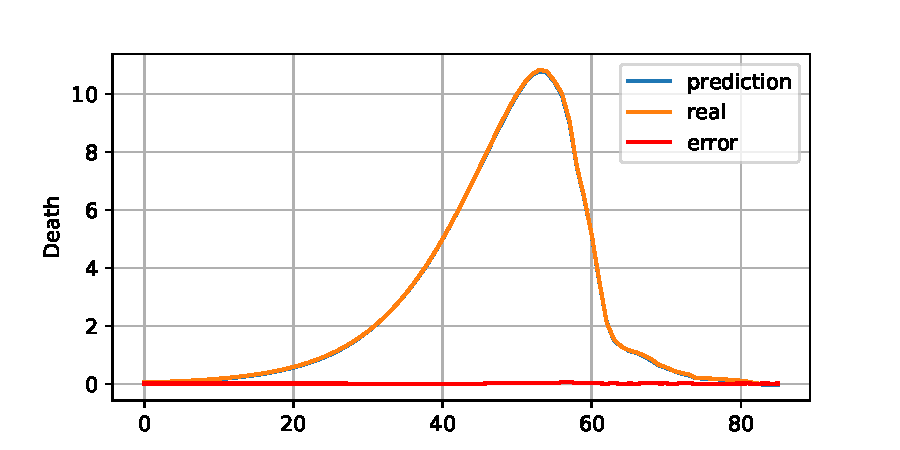
\includegraphics[width=1.0\linewidth]{images/predict/Fig4a.pdf}  
      \caption{Prediction acuracy for deaths.}
      \label{fig:magic-a}
    \end{subfigure}
    \begin{subfigure}{0.49\textwidth}
      \centering
      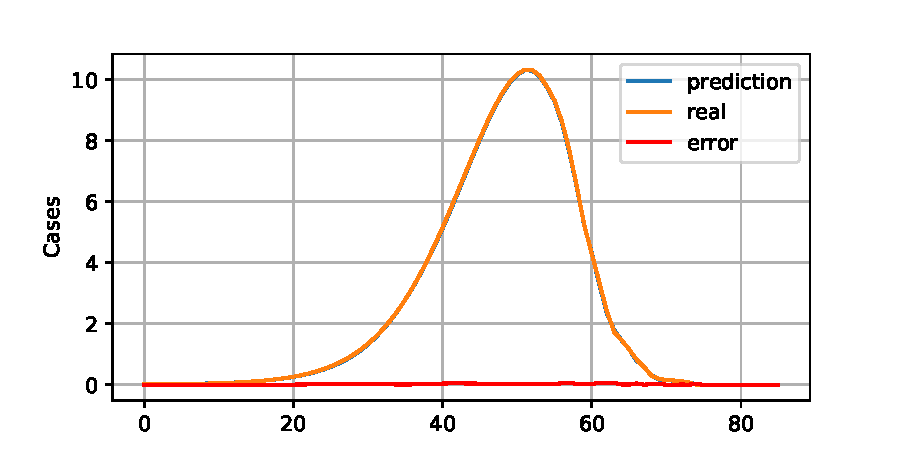
\includegraphics[width=1.0\linewidth]{images/predict/Fig4b.pdf}        
      \caption{Prediction acuracy for cases.}
      \label{fig:magic-b}
    \end{subfigure}

    \caption{Cumulative empirical fits can be very accurately
      predicted with LSTM. The data is taken from 37 U.S. Cities. Our
      comparison showcases that given a model, we can replicate the
      prediction of such models using the model data over time. The
      x-axis represents the days since the first data was fed to the
      model.}
    \label{fig:magic-1}
\end{figure}




\subsection{Realtime-Data Covariate LSTM Prediction}
\label{sec:lstm-covariate}

In this section, we establish that using deep learning can not only be
applied to model predictions but also from real time data. As we want to
evaluate the influence of the risk factors on our prediction framework
using not only models but deep learning algorithms, we have devised a
parameter sweep framework based on LSTM that conducts the prediction
for 110 cities while also considering the risk factors as listed
in Table \ref{tab:risk-factors}. This framework can query any
combination of risk factors as well as not including any, in which
case it defaults to the traditional LSTM algorithm as introduced in
Section \ref{sec:lstm-theory}. Hence, we will answer Questions
\ref{q:2} and \ref{q:3}.

To answer these questions, we chose for our next analysis a date range
between 2020-02-01 and 2020-05-25. We start with a basic LSTM operator
with two layers of LSTM, and initial and final fully connected layers
\citep{Kadupitiya2020-zq}.  For LSTM, we have selected the activation
function based on Rectified Linear Units (RELU). For the last layer
sigmoid is chosen. A drop out rate of 0.2 is used, we use 16 input
nodes, and have a batch size of 110. The  
batch size is the subset size of the training sample (e.g. 110 out of 12540 for a 3 day input length) that is used to train the LSTM during its learning process. The maximum epoch is chosen to be
200. This is the number of steps after we interrupt the learning process. The number of nodes internally is 32. The maximum total number of
samples is 12540 when using 3 days as input length. We use a two-layer
LSTM, as shown in Table \ref{tab:model}. Within our system, we have
the ability to set a number of input days. For this analysis, we have
chosen three different input lengths, namely 3, 4, and 5 days. The
term ``None'' in the output shape means this dimension is
variable. 


\begin{table}[!h]
    \caption{The deep learning parameters used for the model sweep
      creation in as exported by Keras using 1 risk factor. The
      activation function is RELU and the recurrent activation
      function is sigmoid.}
    \label{tab:model}
    \bigskip

    \settowidth{\rotheadsize}{Parameters\quad}

    \begin{footnotesize}
    \centering
    \resizebox{1.0\textwidth}{!}{ 
    \begin{tabular}{|ll|lll|ll|ll|}
    \toprule 
     \rothead{Layer} & \rothead{Type}   &
     \rothead{Output Shape} &  \rothead{Parameters for 0 risk factor}  
                  &  \rothead{Parameters for 1 risk factor} &
     \rothead{Output Shape} &  \rothead{Parameters for 33 risk factors} &
     \rothead{Output Shape} &  \rothead{Parameters for 37 risk factors}\\
    \midrule
    dense & Dense    & (None,1,32) & 96   & 128  &  (None,5,32) & 1152 & (None,5,32) & 1280 \\
    LSTM & LSTM      & (None,1,16) & 3136 & 3136 &  (None,5,16) & 3136 & (None,5,16) & 3136 \\
    LSTM 1 & LSTM   & (None,16)  & 2112  & 2112 &  (None,16)   & 2112 & (None,16)   & 2112 \\
    Dense 1 & Dense & (None,32)  &  544  & 544  &  (None,32)   &  544 & (None,32)   &  544 \\
    Dense 2 & Dense & (None,30)  &  990  & 990  &  (None,30)   &  990 & (None,30)   &  990 \\
    \bottomrule
    \end{tabular}
    } ~\\
    The LSTM contains a total of 6,910 trainable parameters in
    case we include one risk factor. In the case, we do not use any
    risk factor it is 6878, and when we include 33 risk factors, it is
    7934.
    \end{footnotesize}
\end{table}



We have run the training on all 110 cities from our data that
represented each FIPS while not including any risk factors (Question
\ref{q:2}) and running them with a single risk factor while iterating
over all risk factors (Question \ref{q:3}). We then summed up all
absolute errors for the predicted data points over the same time
period and repeated each experiment 10 times. We summarized all the
results in the form of a box-whisker diagram each for deaths and for
cases. We sorted the diagram in such a fashion that the risk factor
that has the model with the lowest error appears first. We preceded
the graph with the experiment labeled as ``NONE'' that which does not
use any risk factors to provide a comparison. The graphs are depicted
in Figures \ref{fig:box-cases} for cases, and \ref{fig:box-death} for
deaths.

\begin{figure}[!p]
    \centering
    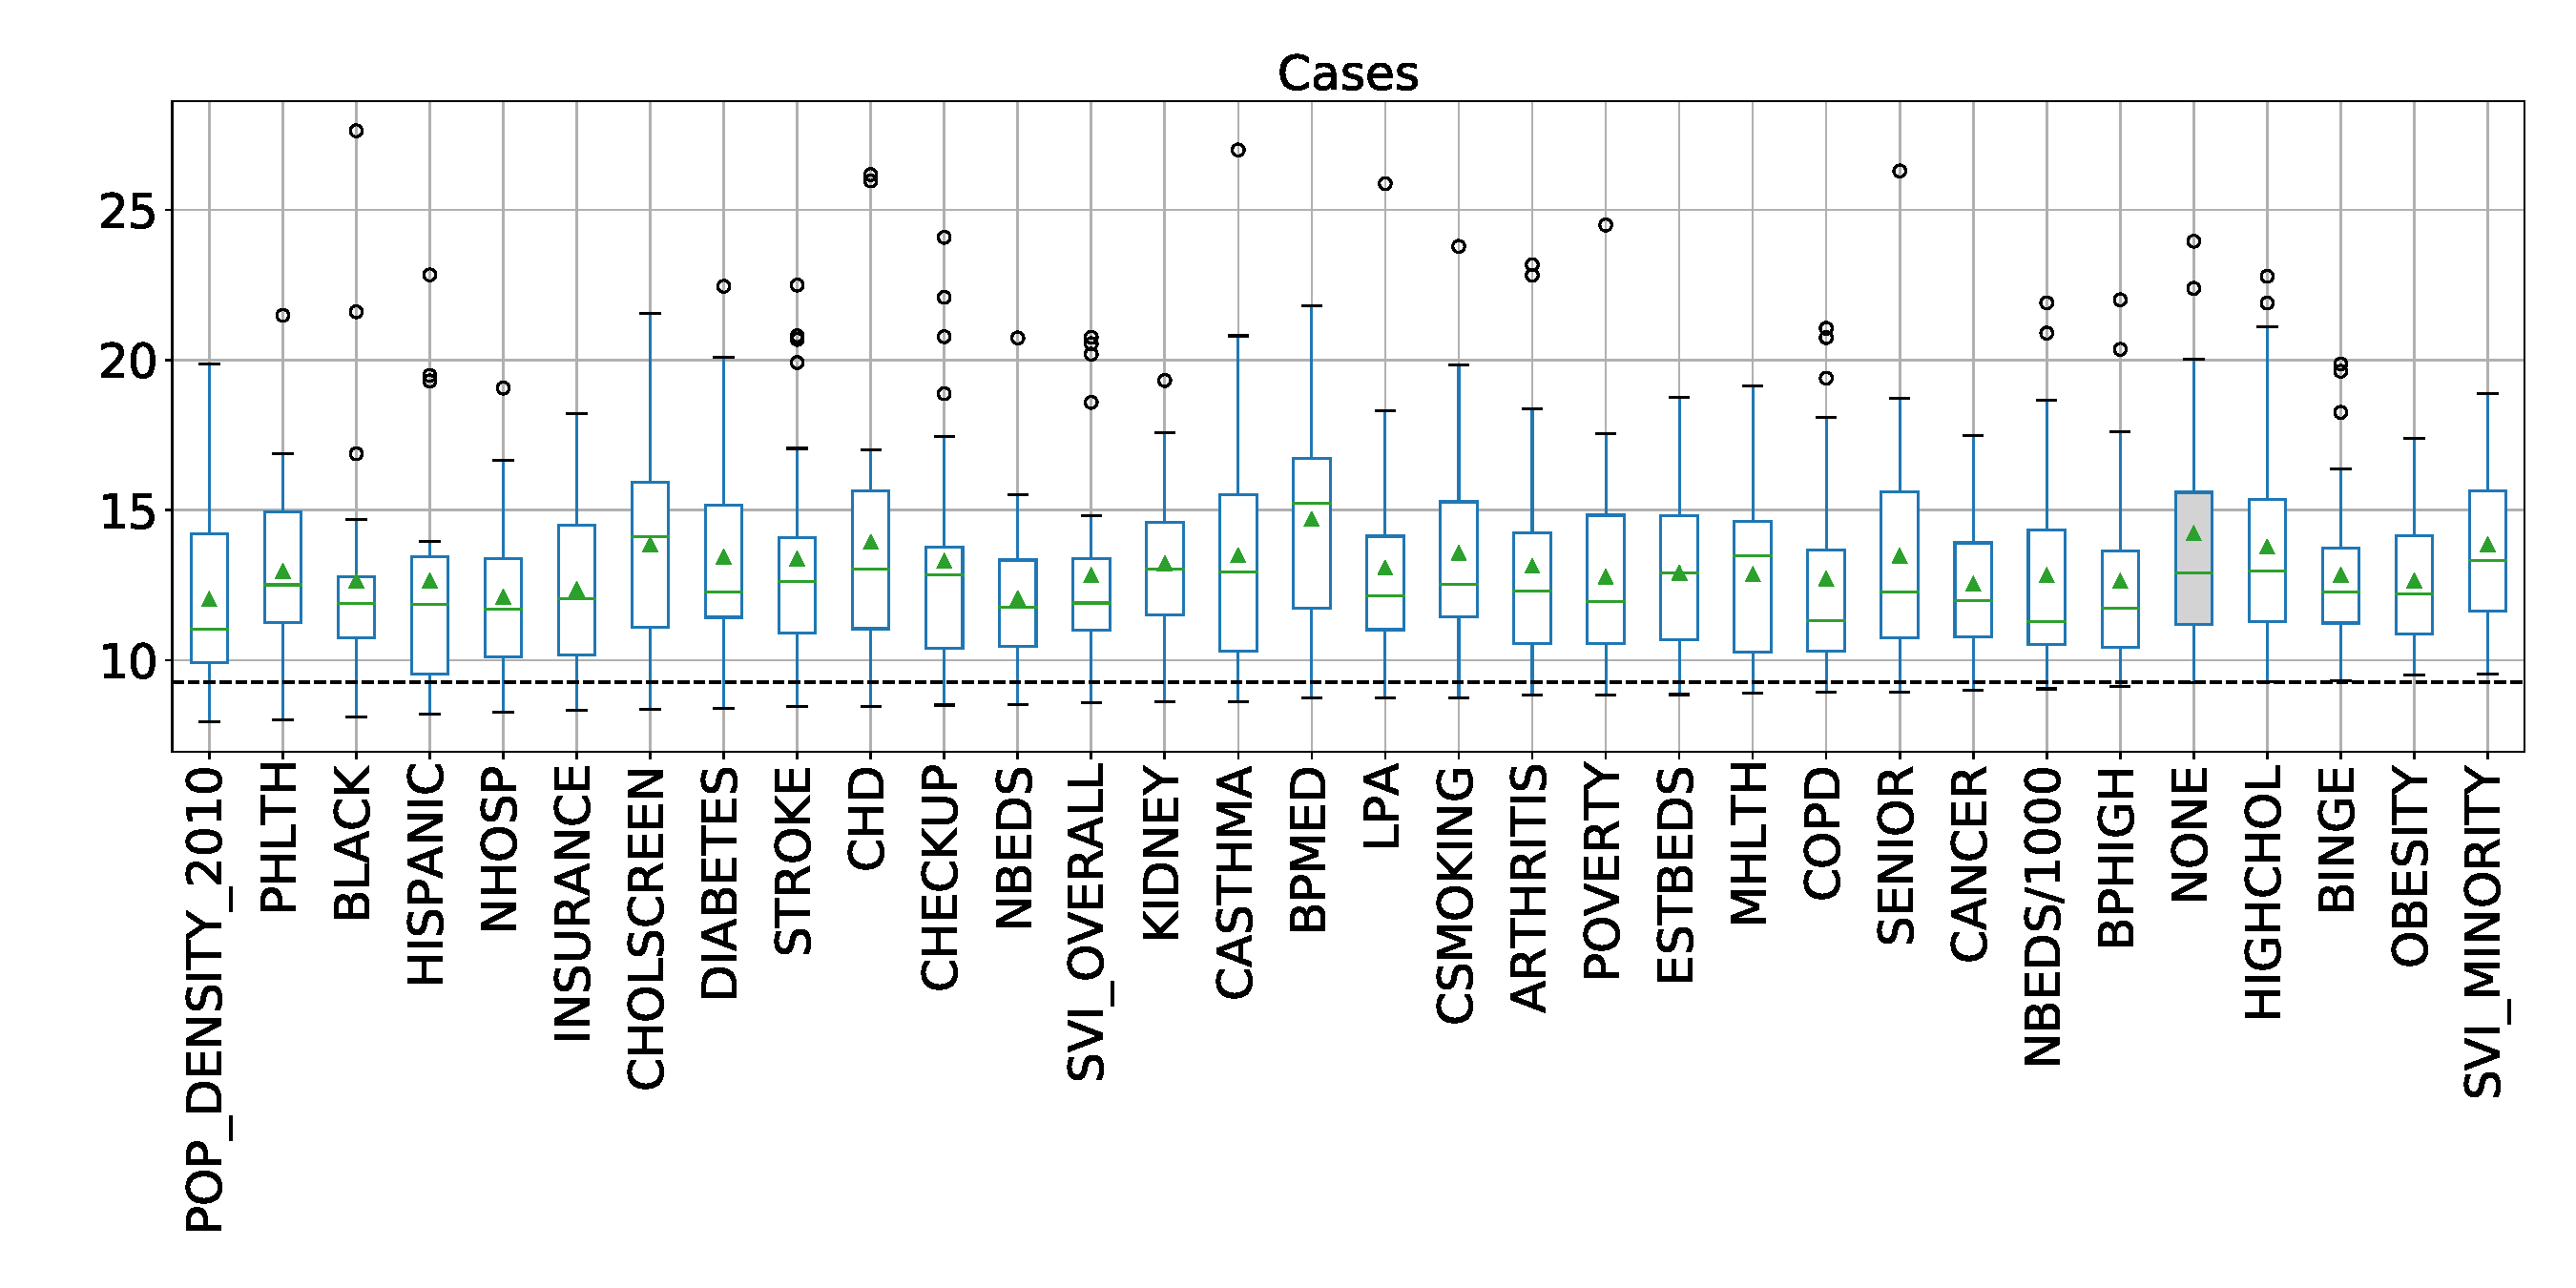
\includegraphics[width=1.0\textwidth]{images/boxwhisker/boxplot_casesNEW2.pdf}
    \vspace{-1cm}
    \caption{Influence of risk factors on the accuracy of the
      prediction of COVID-19 cases. The y-axis represents the
      cumulative error over all input data for the cities.}
    \label{fig:box-cases}
    \bigskip

    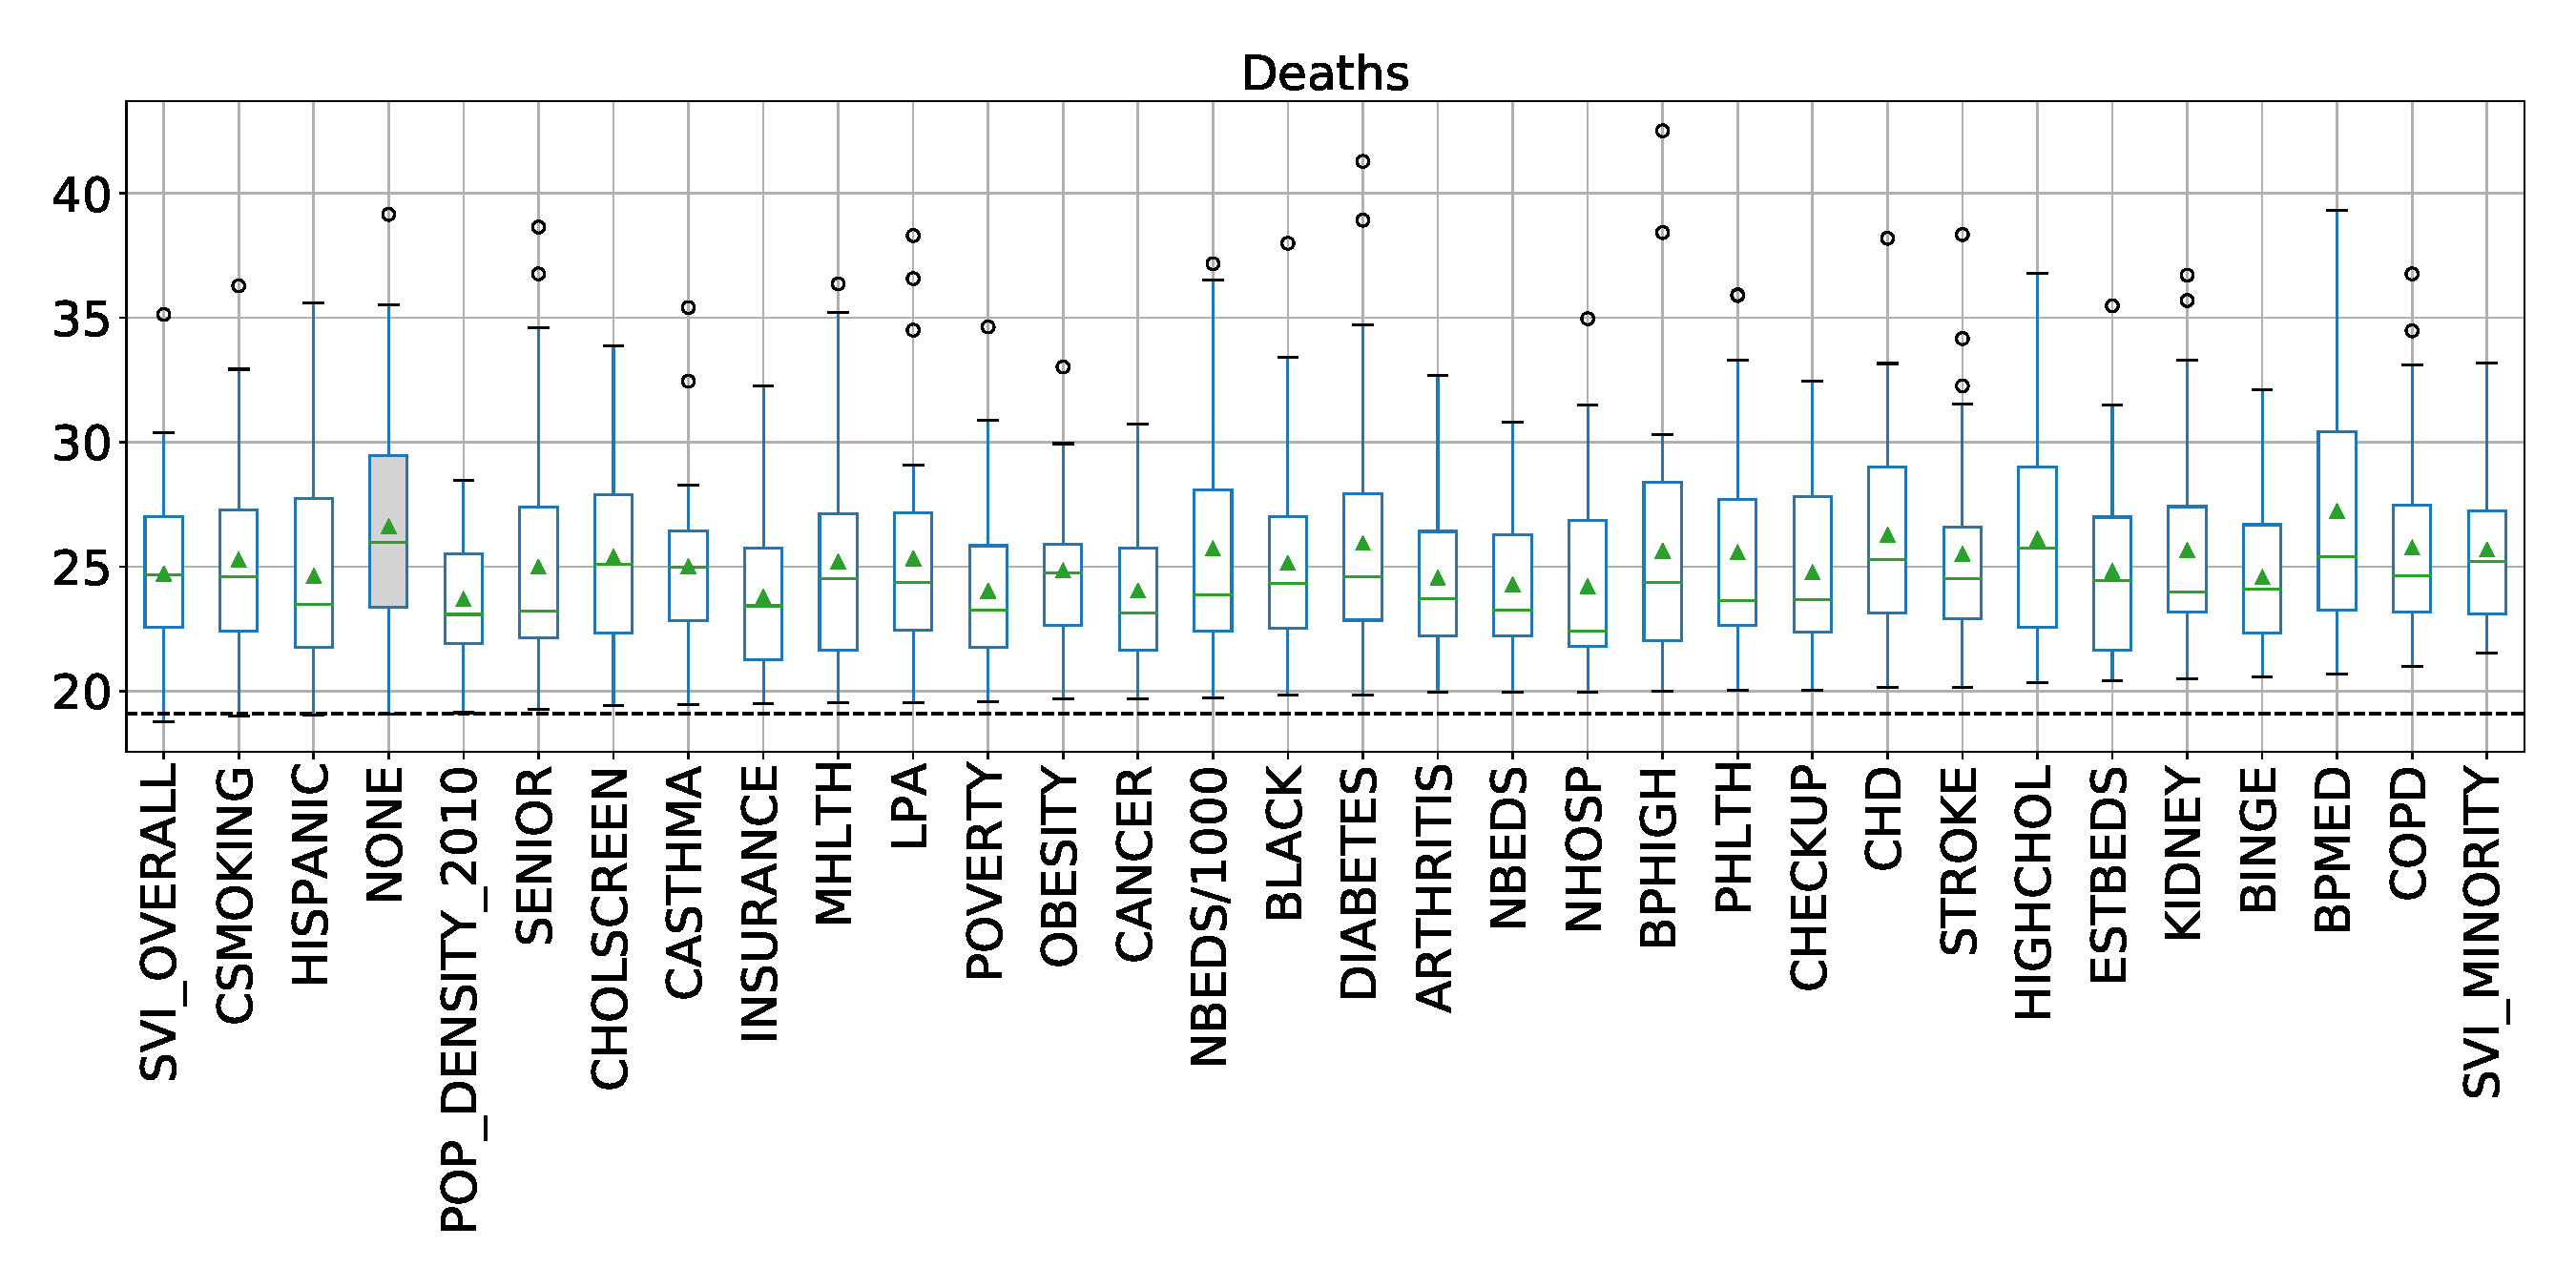
\includegraphics[width=1.0\textwidth]{images/boxwhisker/boxplot_deathNEW2.pdf}
    \vspace{-1cm}
    \caption{Influence of risk factors on the accuracy of the
      prediction of COVID-19 death. The y-axis represents the
      cumulative error over all input data for the cities.}
    \label{fig:box-death}
\end{figure}



Further, the obtained sorted order of the best prediction models by
minimum error based on the risk factors for cases and deaths are as
follows:

\begin{description}

\item[Order for cases sorted by minimum model error:] NONE,
  POP\_DENSITY\_2010, PHLTH, INSURANCE, BLACK,
  HISPANICS, NHOSP, CHOLSCREEN, DIABETES, STROKE,
  CHD, CHECKUP, NBEDS, SVI\_OVERALL, KIDNEY, CASTHMA, BPMED,
  LPA, CSMOKING, ARTHRITIS, POVERTY, ESTBEDS, MHLTH, SENIOR, COPD,
  CANCER, NBEDS/1000, BPHIGH, HIGHCHOL, BINGE, OBESITY, SVI\_MINORITY

\item[Order for deaths sorted by minimum model error:] NONE,
  SVI\_OVERALL, CSMOKING, HISPANICS, POP\_DENSITY\_2010,
  SENIOR, CHOLSCREEN, CASTHMA, INSURANCE, MHLTH, LPA,
  POVERTY, OBESITY, CANCER, BLACK, NBEDS/1000, DIABETES, ARTHRITIS,
  NBEDS, NHOSP, BPHIGH, CHECKUP, PHLTH, CHD, STROKE, HIGHCHOL,
  ESTBEDS, KIDNEY, BINGE, BPMED, COPD, SVI\_MINORITY
\end{description}

We show the errors and the association with a risk factors in Table
 \ref{tab:top-1-cases} and \ref{tab:top-1-deaths}. In the tables we include the following columns (a) the Risk Factor (b) the root mean square error of all models for this risk factor (c) the minimum cumulative error by risk factor and (d) the number of days that wer used as input and identified to relate to the model with the minimum cumulative error. The table has in the first column the rank this particular model comperes to all other models with minimal risk factor. 
The rank was obtained by sorting the best model for each risk factor. 
We display two tables. One for cases (Table \ref{tab:top-1-cases} and one for deaths (Table \ref{tab:top-1-cases}).

We see that in our experiment, almost all risk factors lead to an increased
model prediction accuracy for cases.  We note that by including
factors such as population density, physical health Insurance,
population breakdown by ethnicity, number of hospitals, and diabetes,
lead to better overall predictions for cases. 
We also see that
many of these factors perform better on average.

\begin{table}[!p]
\caption{Best models for cases for each risk factor and their respective
  errors. The model that uses no risk factor is highlighted in grey. We present the Root Mean Square Error (RMSE), the cumulative error and how many days as input were used for this corresponding model.}
\label{tab:top-1-cases}
\bigskip
\centering
%\resizebox{1.0\textwidth}{!}{ 
\begin{tabular}{rrrrrlrl}
\toprule
 \makecell{Place/\\Rank} & 
\makecell{Risk Factor} &  
\makecell{RMSE\\Cases} &  
  \makecell[r]{Minimum\\Cumu-\\lative \\Error for \\Cases by\\Risk Factor} & 
 \makecell[r]{Number of \\Days as \\Input} \\
\midrule

1	&	POP\_DENSITY\_2010	&	0.055443	&	7.94	&	5	 \\
2	&	PHLTH	&	0.054795	&	8.01	&	3	 \\
3	&	BLACK	&	0.055028	&	8.12	&	4	 \\
4	&	HISPANIC	&	0.056061	&	8.22	&	5	 \\
5	&	NHOSP	&	0.054621	&	8.26	&	3	 \\
6	&	INSURANCE	&	0.054557	&	8.34	&	3	 \\
7	&	CHOLSCREEN	&	0.054712	&	8.37	&	3	 \\
8	&	DIABETES	&	0.054586	&	8.4	&	5	 \\
9	&	STROKE	&	0.05416	&	8.45	&	4	 \\
10	&	CHD	&	0.054027	&	8.46	&	5	 \\
11	&	CHECKUP	&	0.054927	&	8.51	&	5	 \\
12	&	NBEDS	&	0.054146	&	8.54	&	5	 \\
13	&	SVI\_OVERALL	&	0.054795	&	8.58	&	5	 \\
14	&	KIDNEY	&	0.0546	&	8.61	&	5	 \\
15	&	CASTHMA	&	0.055089	&	8.63	&	5	 \\
16	&	BPMED	&	0.054685	&	8.74	&	3	 \\
17	&	LPA	&	0.054323	&	8.75	&	5	 \\
18	&	CSMOKING	&	0.053716	&	8.75	&	5	 \\
19	&	ARTHRITIS	&	0.054053	&	8.83	&	3	 \\
20	&	POVERTY	&	0.055029	&	8.84	&	3	 \\
21	&	ESTBEDS	&	0.054545	&	8.86	&	4	 \\
22	&	MHLTH	&	0.054864	&	8.9	&	3	 \\
23	&	COPD	&	0.055589	&	8.93	&	4	 \\
24	&	SENIOR	&	0.055079	&	8.93	&	3	 \\
25	&	CANCER	&	0.0545	&	8.99	&	3	 \\
26	&	NBEDS/1000	&	0.054397	&	9.05	&	3	 \\
27	&	BPHIGH	&	0.054609	&	9.13	&	4	 \\
\rowcolor{black!5} 28	&	NONE	&	0.054868	&	9.26	&	3	 \\
29	&	HIGHCHOL	&	0.056429	&	9.28	&	3	 \\
30	&	BINGE	&	0.054317	&	9.32	&	5	 \\
31	&	OBESITY	&	0.054469	&	9.5	&	3	 \\
32	&	SVI\_MINORITY	&	0.055094	&	9.54	&	4	 \\
\bottomrule
\end{tabular}
%}
\end{table}

\begin{table}[!p]
\caption{Best models for deaths for each risk factor and their respective
  errors. The model that uses no risk factor is highlighted in grey.
  We present the Root Mean Square Error (RMSE), the cumulative error and how many days as input were used for this corresponding model.
  }
\label{tab:top-1-deaths}
\bigskip
\centering
%\resizebox{1.0\textwidth}{!}{ 
\begin{tabular}{rrrrrlrl}
\toprule
 \makecell{Place/\\Rank} & 
\makecell{Risk Factor} &  
\makecell{RMSE\\Deaths} &  
\makecell[r]{Minimum\\Cumu-\\lative \\Error for \\Deaths by\\Risk Factor} &  
 \makecell[r]{Number of \\Days as \\Input} \\
\midrule
1	&	SVI\_OVERALL	&	0.067457	&	18.75	&	5	 \\
2	&	CSMOKING	&	0.066898	&	19.01	&	5	 \\
3	&	HISPANIC	&	0.067489	&	19.04	&	5	 \\
\rowcolor{black!5} 4	&	NONE	&	0.06696	&	19.09	&	4	 \\
5	&	POP\_DENSITY\_2010	&	0.066968	&	19.13	&	4	 \\
6	&	SENIOR	&	0.068498	&	19.27	&	3	 \\
7	&	CHOLSCREEN	&	0.067859	&	19.43	&	5	 \\
8	&	CASTHMA	&	0.066952	&	19.46	&	5	 \\
9	&	INSURANCE	&	0.067127	&	19.48	&	5	 \\
10	&	MHLTH	&	0.068742	&	19.53	&	3	 \\
11	&	LPA	&	0.067149	&	19.54	&	5	 \\
12	&	POVERTY	&	0.067267	&	19.57	&	5	 \\
13	&	OBESITY	&	0.067123	&	19.68	&	5	 \\
14	&	CANCER	&	0.068363	&	19.70	&	3	 \\
15	&	NBEDS/1000	&	0.06752	&	19.73	&	5	 \\
16	&	BLACK	&	0.068352	&	19.83	&	3	 \\
17	&	DIABETES	&	0.067636	&	19.84	&	5	 \\
18	&	ARTHRITIS	&	0.066927	&	19.94	&	4	 \\
19	&	NBEDS	&	0.066879	&	19.95	&	4	 \\
20	&	NHOSP	&	0.067391	&	19.95	&	5	 \\
21	&	BPHIGH	&	0.067799	&	19.99	&	5	 \\
22	&	PHLTH	&	0.068737	&	20.02	&	3	 \\
23	&	CHECKUP	&	0.067543	&	20.02	&	5	 \\
24	&	CHD	&	0.06874	&	20.15	&	3	 \\
25	&	STROKE	&	0.066906	&	20.16	&	4	 \\
26	&	HIGHCHOL	&	0.068557	&	20.35	&	3	 \\
27	&	ESTBEDS	&	0.067052	&	20.42	&	4	 \\
28	&	KIDNEY	&	0.068948	&	20.49	&	3	 \\
29	&	BINGE	&	0.067447	&	20.56	&	5	 \\
30	&	BPMED	&	0.067399	&	20.69	&	5	 \\
31	&	COPD	&	0.06745	&	20.98	&	5	 \\
32	&	SVI\_MINORITY	&	0.067443	&	21.53	&	4	 \\
\bottomrule
\end{tabular}
%}
\end{table}

We observed a different scenario for deaths, in which we only
identified two risk factors, namely the Social Vulnerability Index
(SVI) and chain-smoking, that, when integrated into our deep learning
model, leads to better prediction results. However, the accuracy of
the overall prediction of deaths is far less precise than that of the
cases. To showcase this, we have included Figures
\ref{fig:error-case-popdensity} and \ref{fig:error-death-popdensity}
that show the respective errors.

\begin{figure}[!h]
  \begin{subfigure}{.49\textwidth}
    \centering
    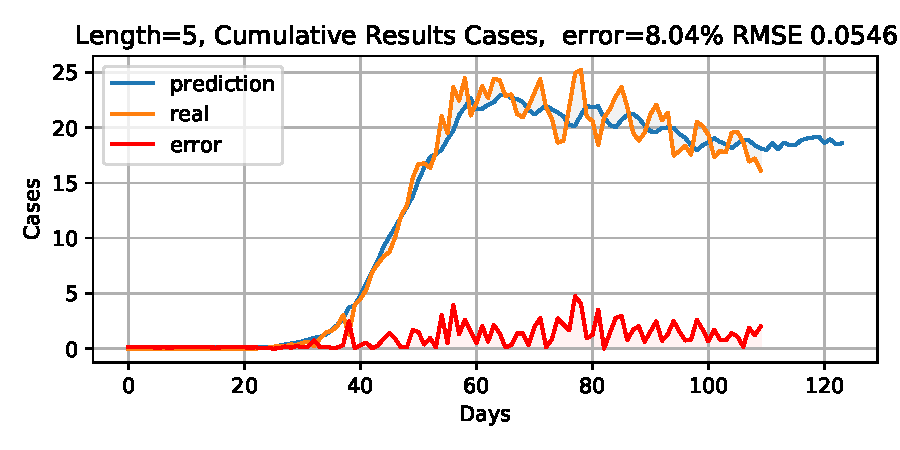
\includegraphics[width=1.0\textwidth]{images/predict/Length_5-fields_pop_density_2010-Cumulative-Cases.pdf}
    %\vspace{-1cm}
    \caption{Model prediction error cases.}
    \label{fig:error-case-popdensity}
  \end{subfigure}
  \begin{subfigure}{.49\textwidth}
    \centering
    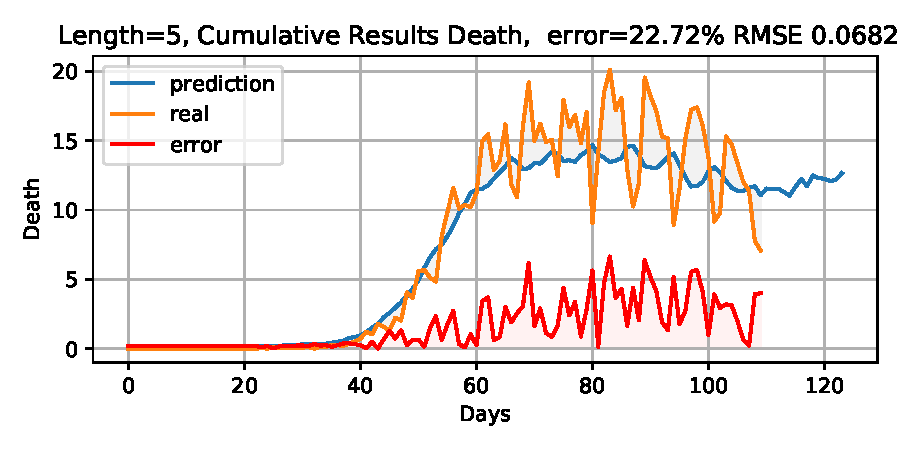
\includegraphics[width=1.0\textwidth]{images/predict/Length_5-fields_pop_density_2010-Cumulative-Death.pdf}
    %\vspace{-1cm}
    \caption{Model prediction error deaths.}
    \label{fig:error-death-popdensity}
    \end{subfigure}

    \caption{Model prediction error for cumulative deaths when
      including one risk factor POP\_DENSITY\_2010
      in addition to the past number of cases and deaths.}
    \label{fig:error-death-popdensity-both}
  
    
\end{figure}


This can be explained by our input data distribution between cases and deaths in which we noted higher
fluctuations relative to the overall value in cases of deaths. 
A mitigation to this issue
would be using a seven day average over the analyzed period. However,
we have not done this on purpose for this analysis as we wanted to
identify how a covariate enhanced LSTM behaves that includes risk
factors based on the daily fluctuations. This was done to avoid and
showcase any needed preproccessing on the data and to identify the
capability of the deep learning framework while adapting to the
fluctuations without any special activities. Previously, we have
already shown in Section \ref{sec:emperical} that for smooth data
inputs the prediction is very accurate.  Using fluctuation data allows
our framework for an automated ingest of data on a daily basis to
enable data fusion of new cases and death information. Hence, we can
re-train the model with new incoming data every day. Through repeated
training experiments, we found the LSTM hyperparameters such as epochs
and dropout values that work well for our experiments.

We conducted an additional analysis and plotted the top 10 best
cumulative prediction model errors for each risk factor in
Figure \label{fig:place-top10} for cases and deaths.  The horizontal
black line shows the first occurrence of no risk factor being used.

Notably, we identified that a jump occurs when we sort the top 10
model predictions at around 330 models from a total of 3400
automatically generated models. This also underscores the need to run
our deep learning model multiple times to obtain best parameter
candidates.  Furthermore, we see that the cumulative error for cases
is about half the size as for death. This is caused by cases having a
larger number of samples than those from deaths.

% In case of cases we also see a drop in the better
% model predictions. 



\begin{figure}[!htbp]
%    \begin{minipage}{.45\textwidth}
%        \centering
%        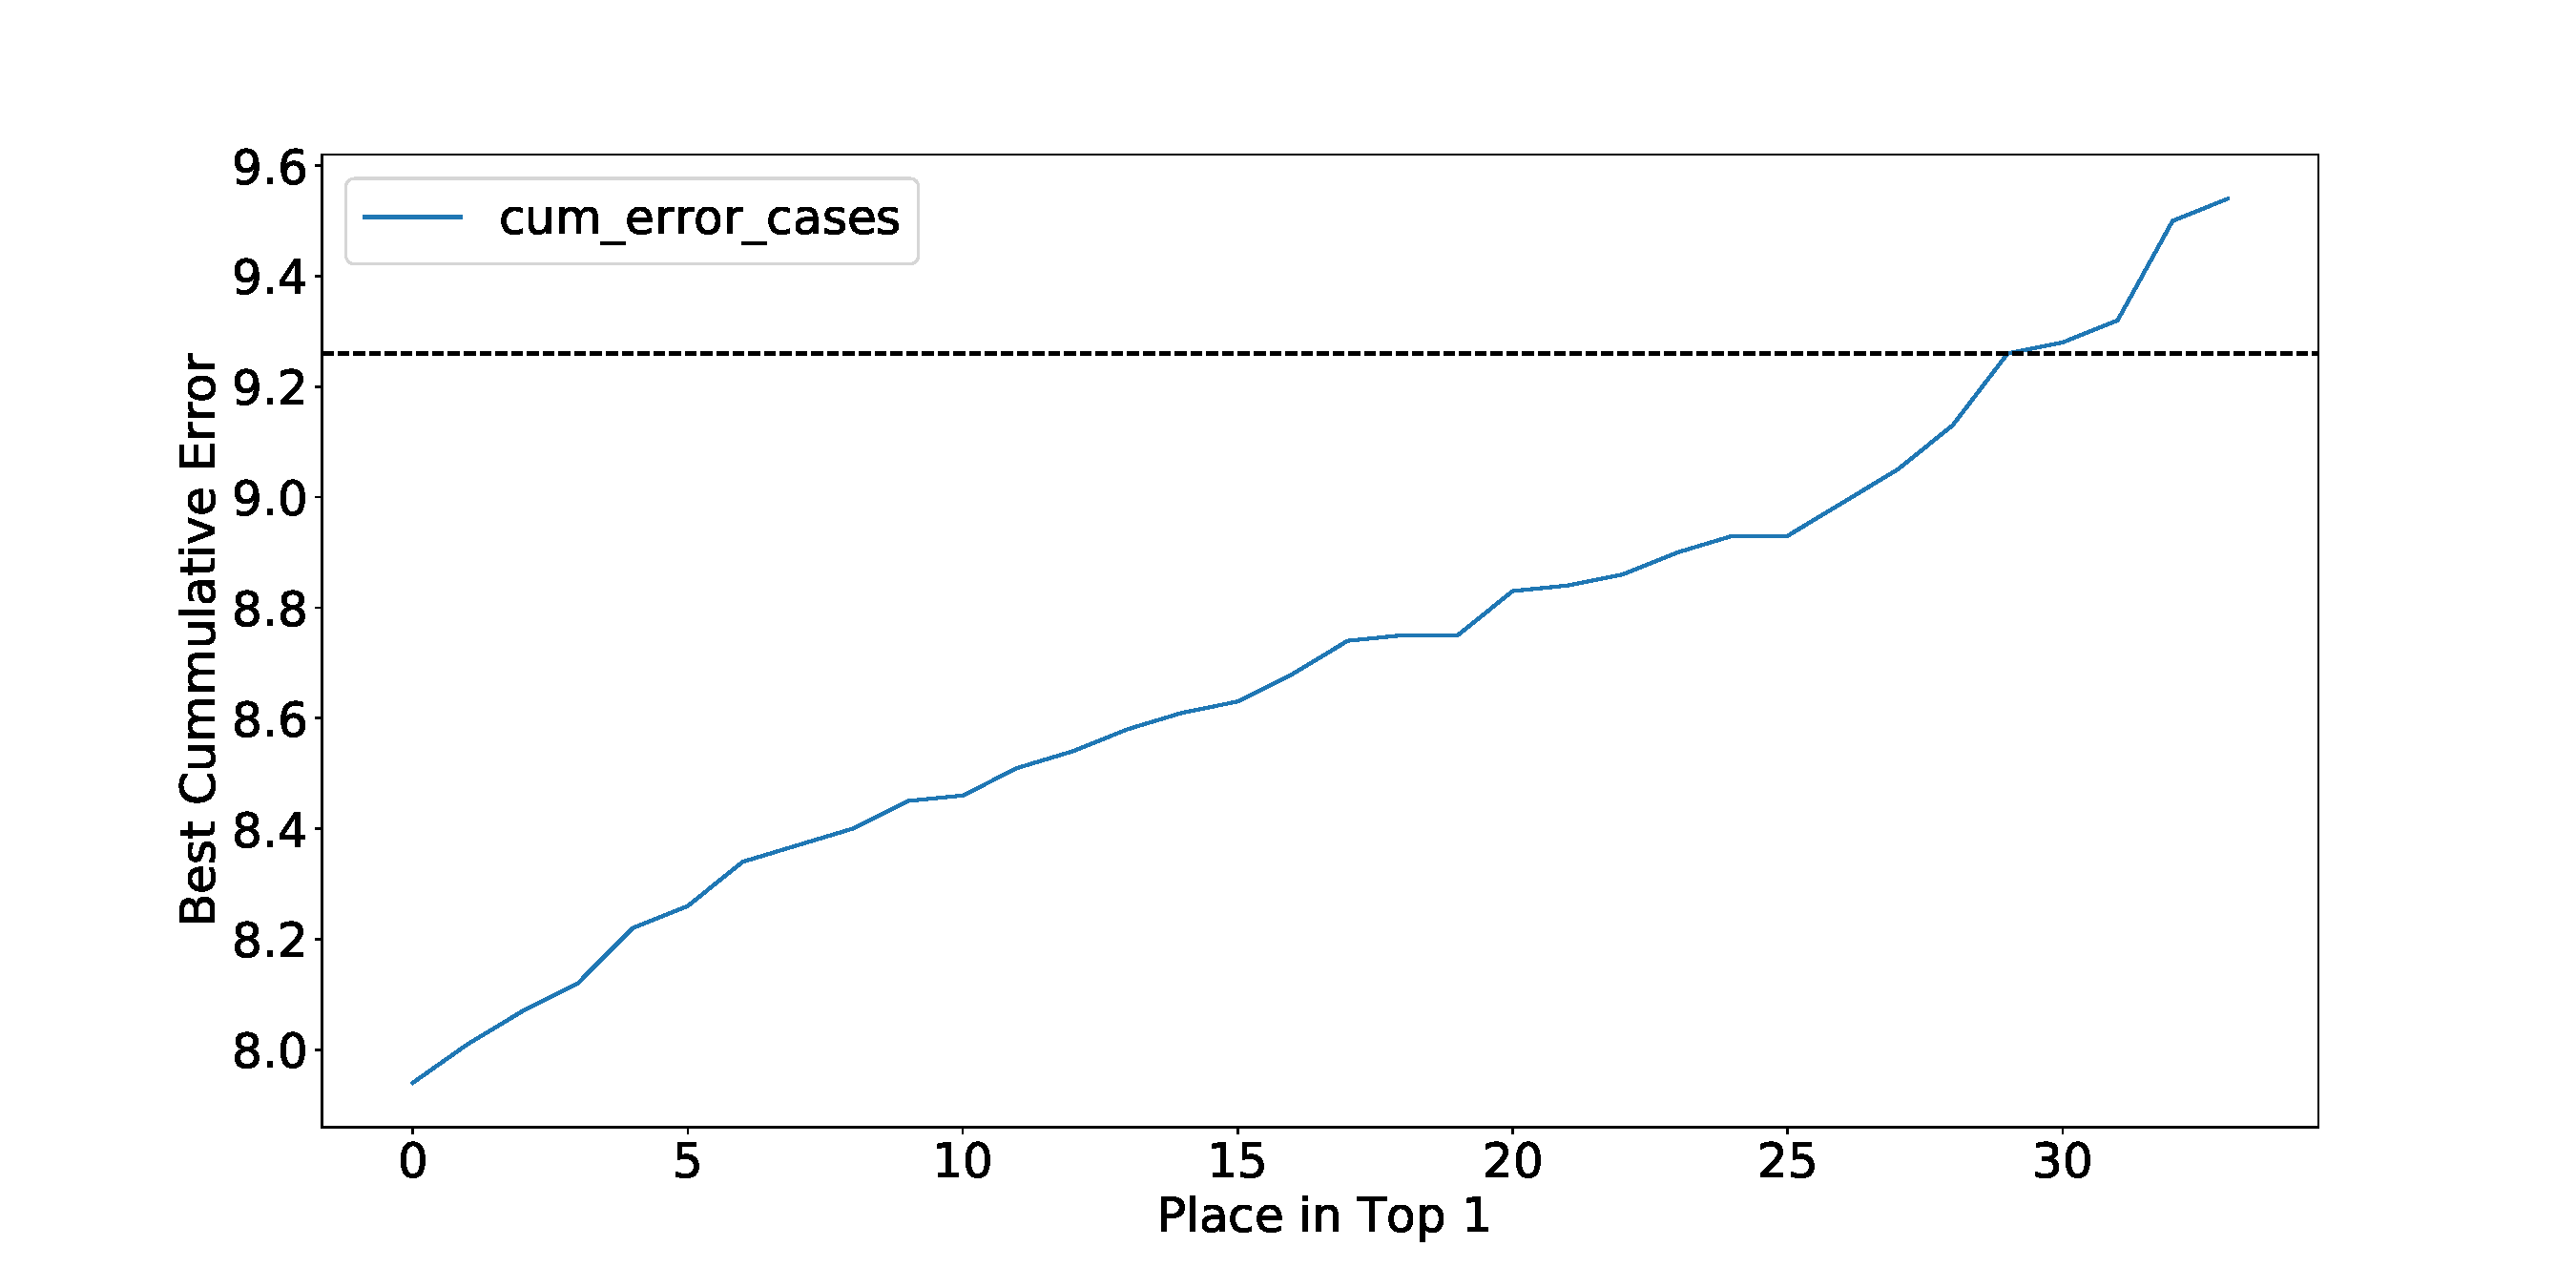
\includegraphics[width=1.0\textwidth]{images/predict/PlaceTop1_Cases.pdf}
%        \vspace{-1cm}
%        \caption{Best predictions for cases over all risk factors.}
%        \label{fig:place-top1-cases}
%
%    \end{minipage}
%    \ \
%    \begin{minipage}{0.45\textwidth}
%        \centering
%        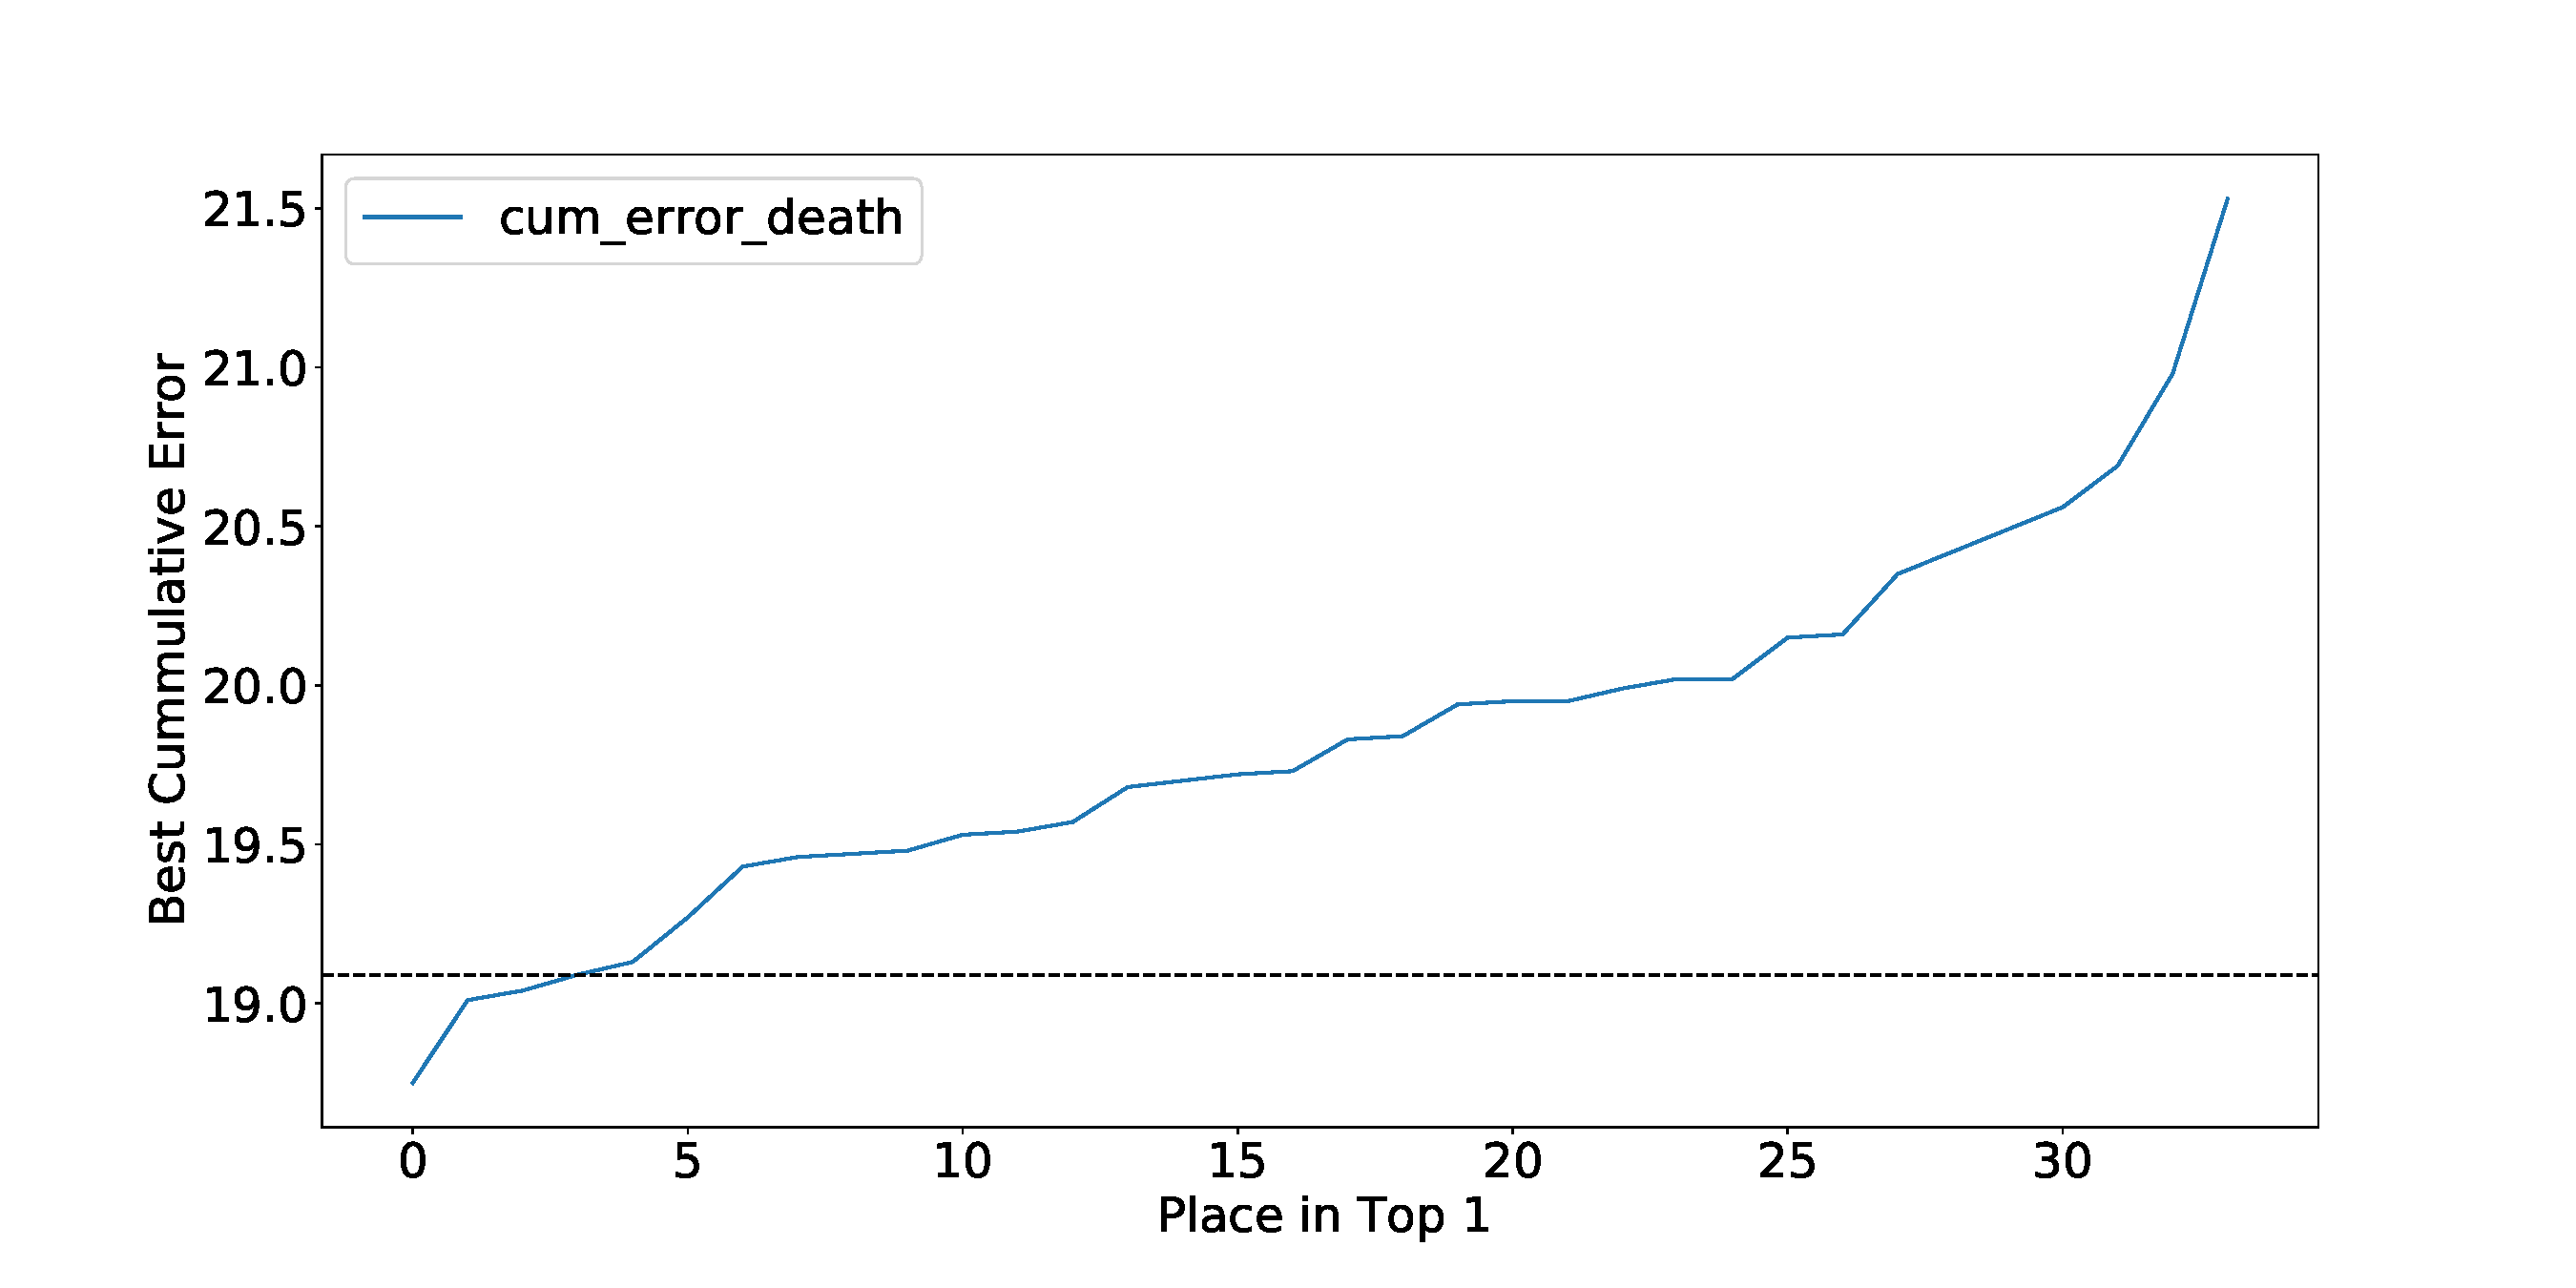
\includegraphics[width=1.0\textwidth]{images/predict/PlaceTop1_Death.pdf}
%        \vspace{-1cm}
%        \caption{Best predictions for deaths over all risk factors.}
%        \label{fig:place-top1-death}
%    \end{minipage}

%    \begin{minipage}{.45\textwidth}
%        \centering
%        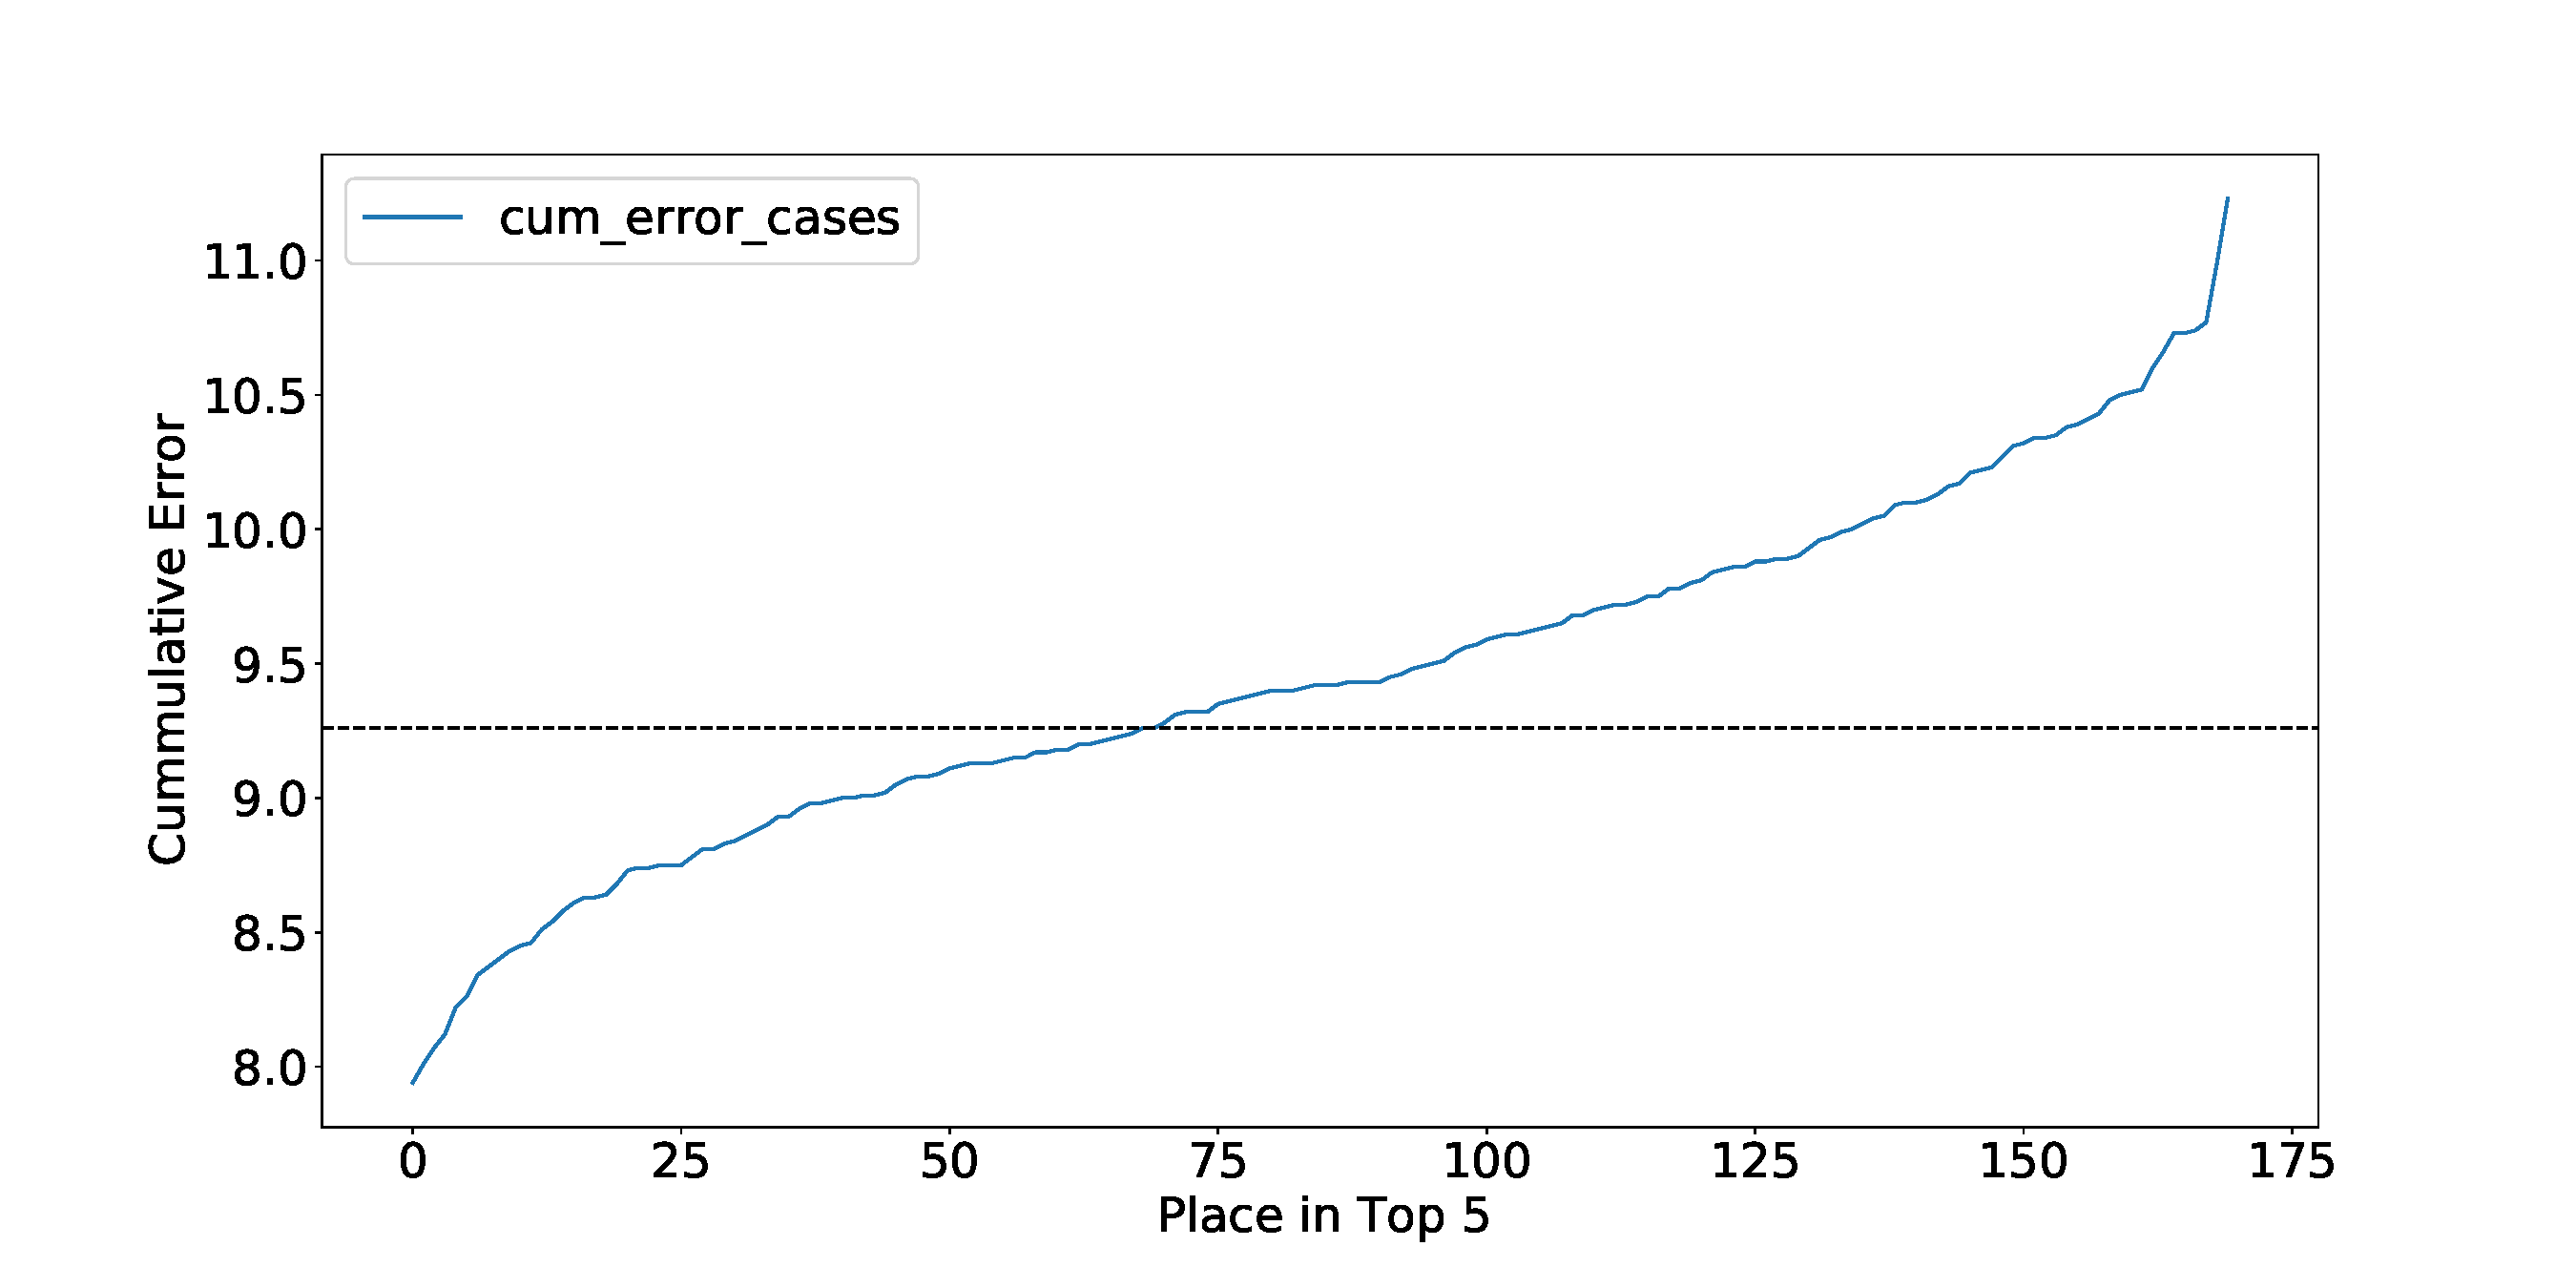
\includegraphics[width=1.0\textwidth]{images/predict/PlaceTop5_Cases.pdf}
%        \vspace{-1cm}
%        \caption{Top 5 predictions from all cases over all risk factors.}
%        \label{fig:place-top5-cases}
%    \end{minipage}
%    \ \
%    \begin{minipage}{.45\textwidth}
%        \centering
%        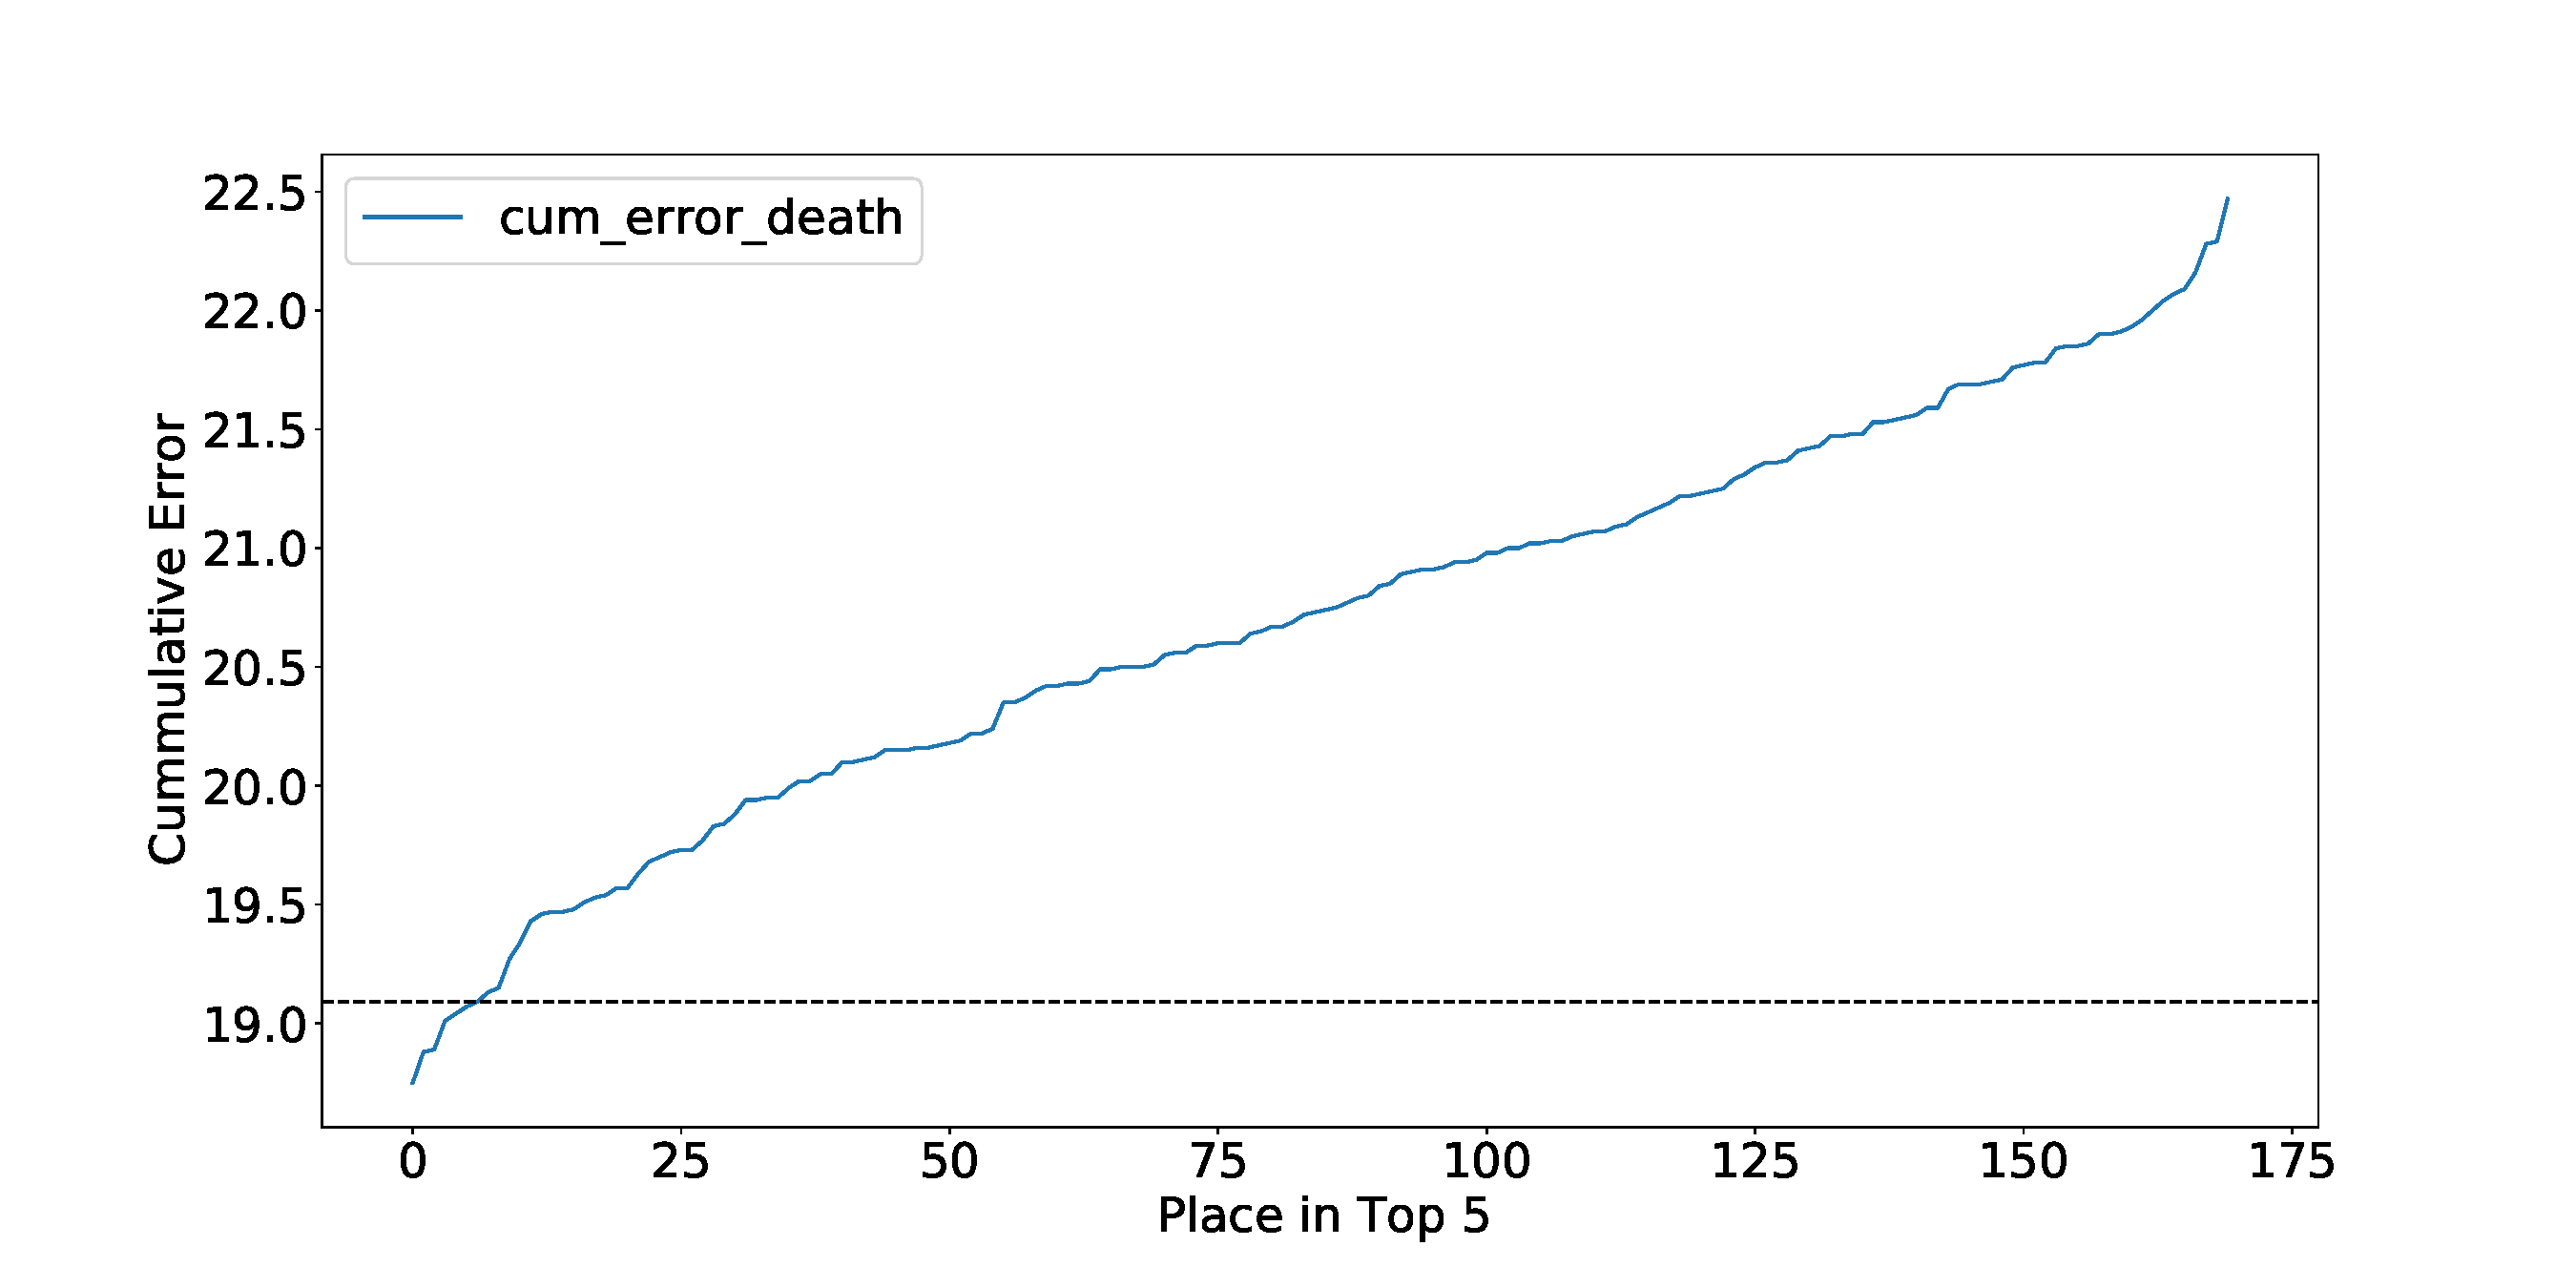
\includegraphics[width=1.0\textwidth]{images/predict/PlaceTop5_Death.pdf}
%        \vspace{-1cm}
%        \caption{Top 5 predictions from all deaths  over all risk factors.}
%        \label{fig:place-top5-death}
%    \end{minipage}
    \begin{subfigure}{.95\textwidth}
        \centering
        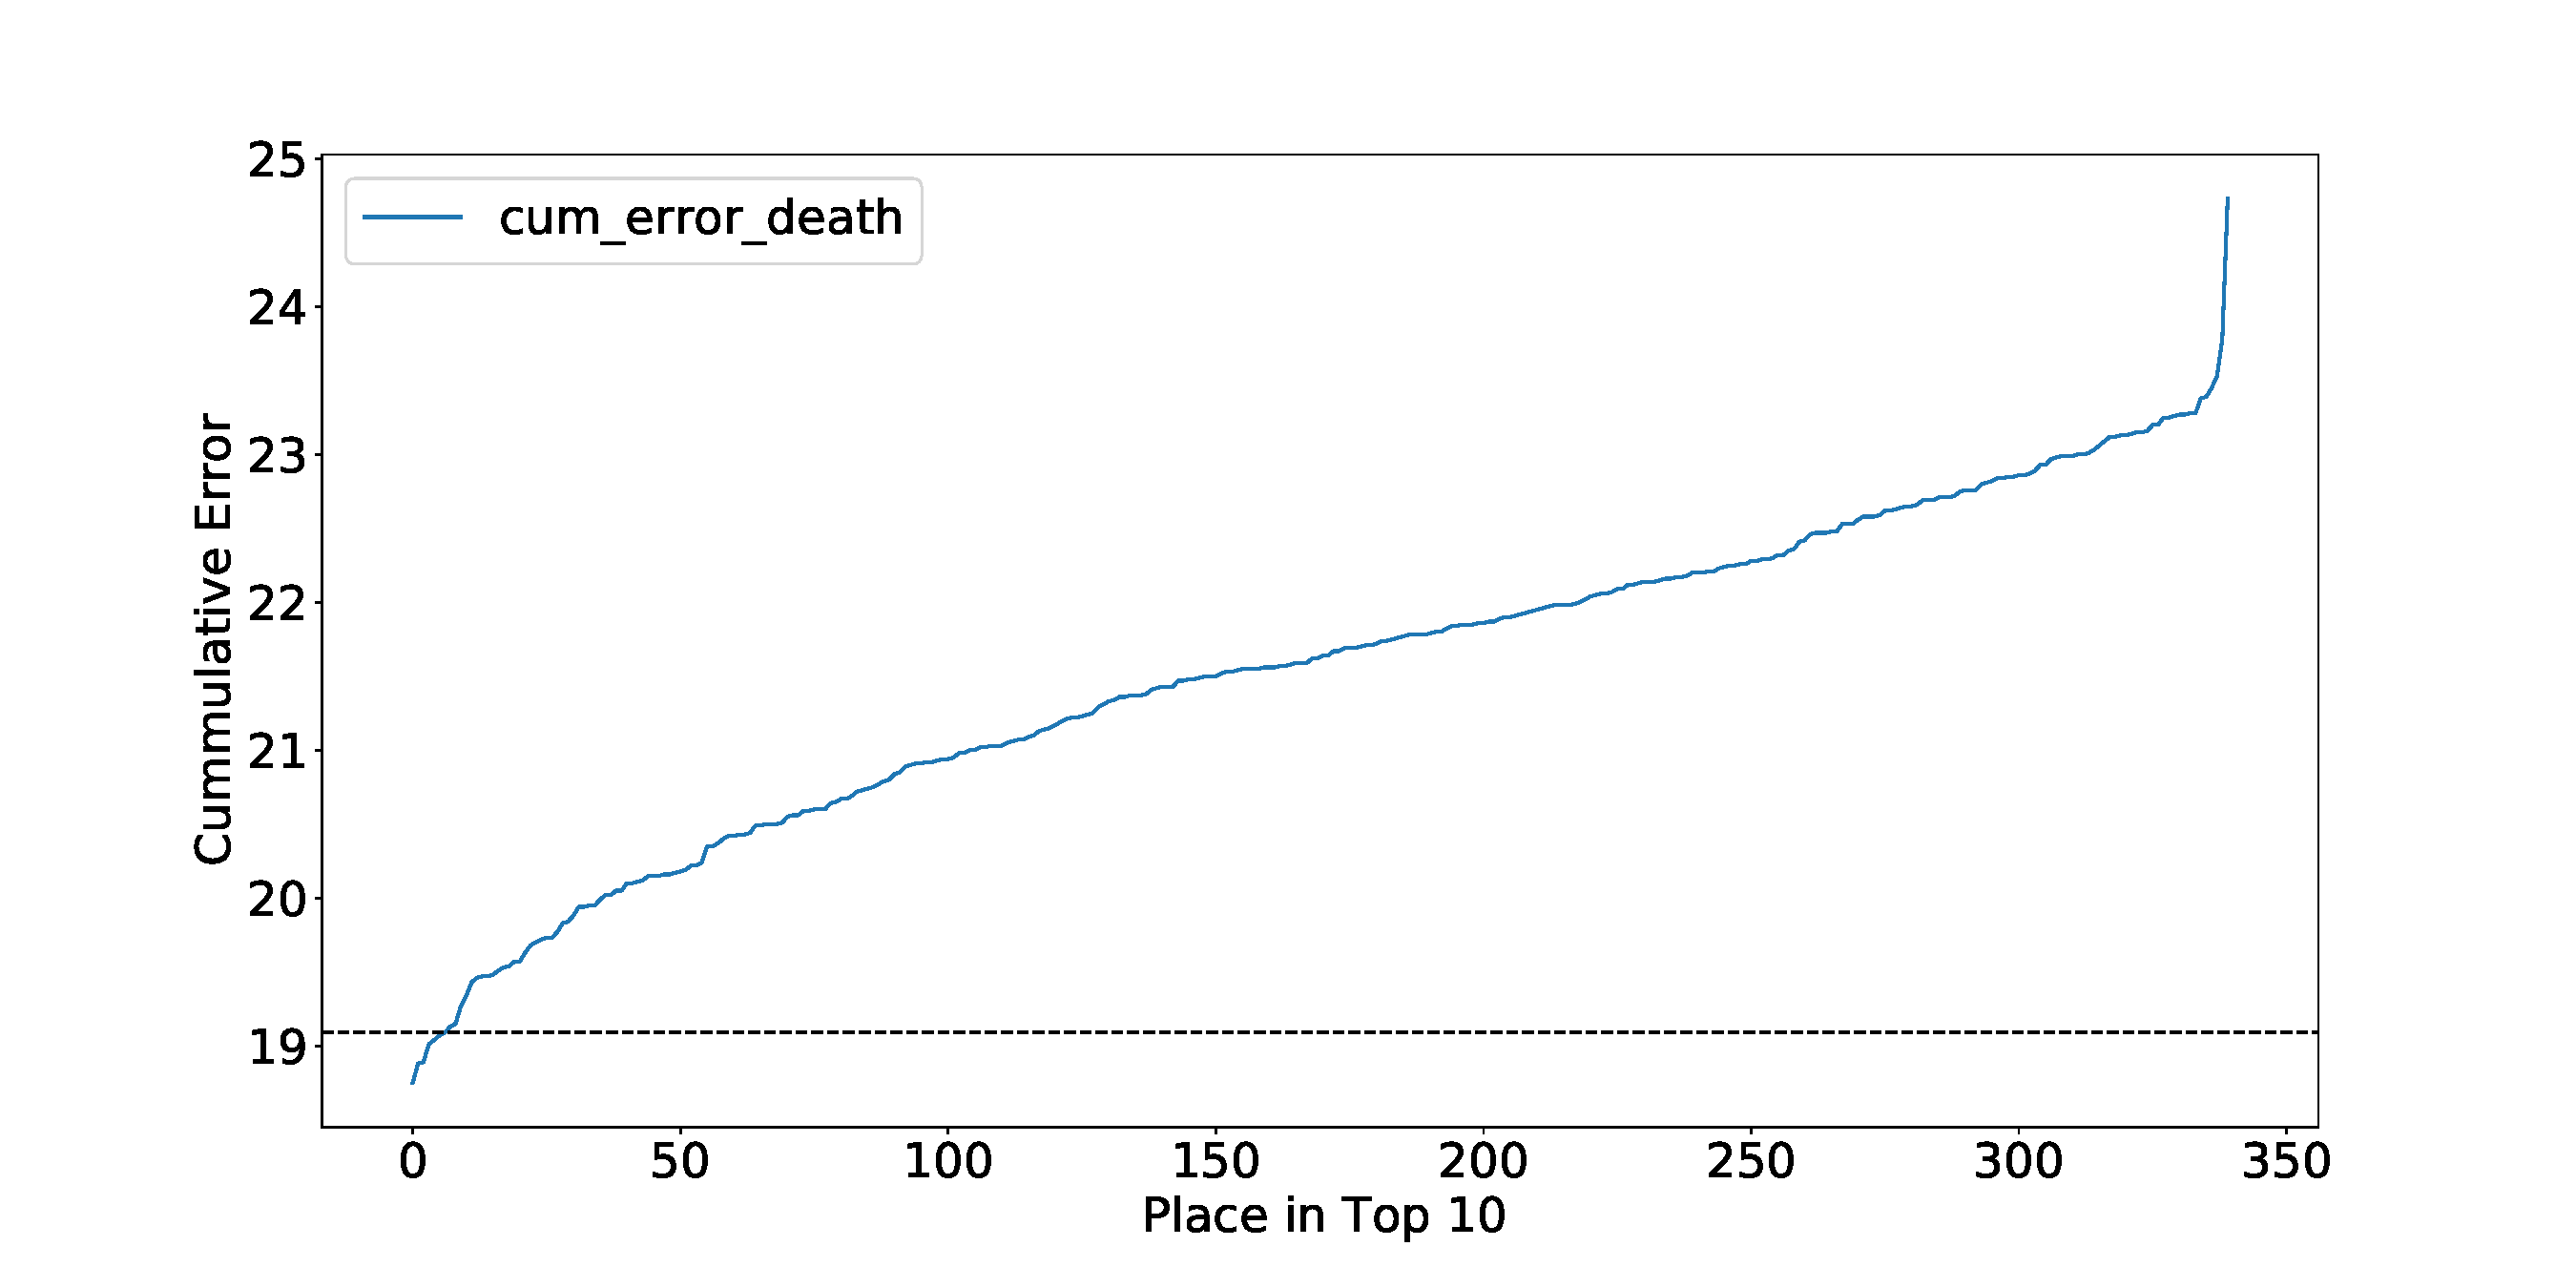
\includegraphics[width=1.0\textwidth]{images/predict/PlaceTop10_Death.pdf}
        \caption{Cumulative error for deaths.}
        \label{fig:place-top10-death}
    \end{subfigure}
    \begin{subfigure}{.95\textwidth}
        \centering
        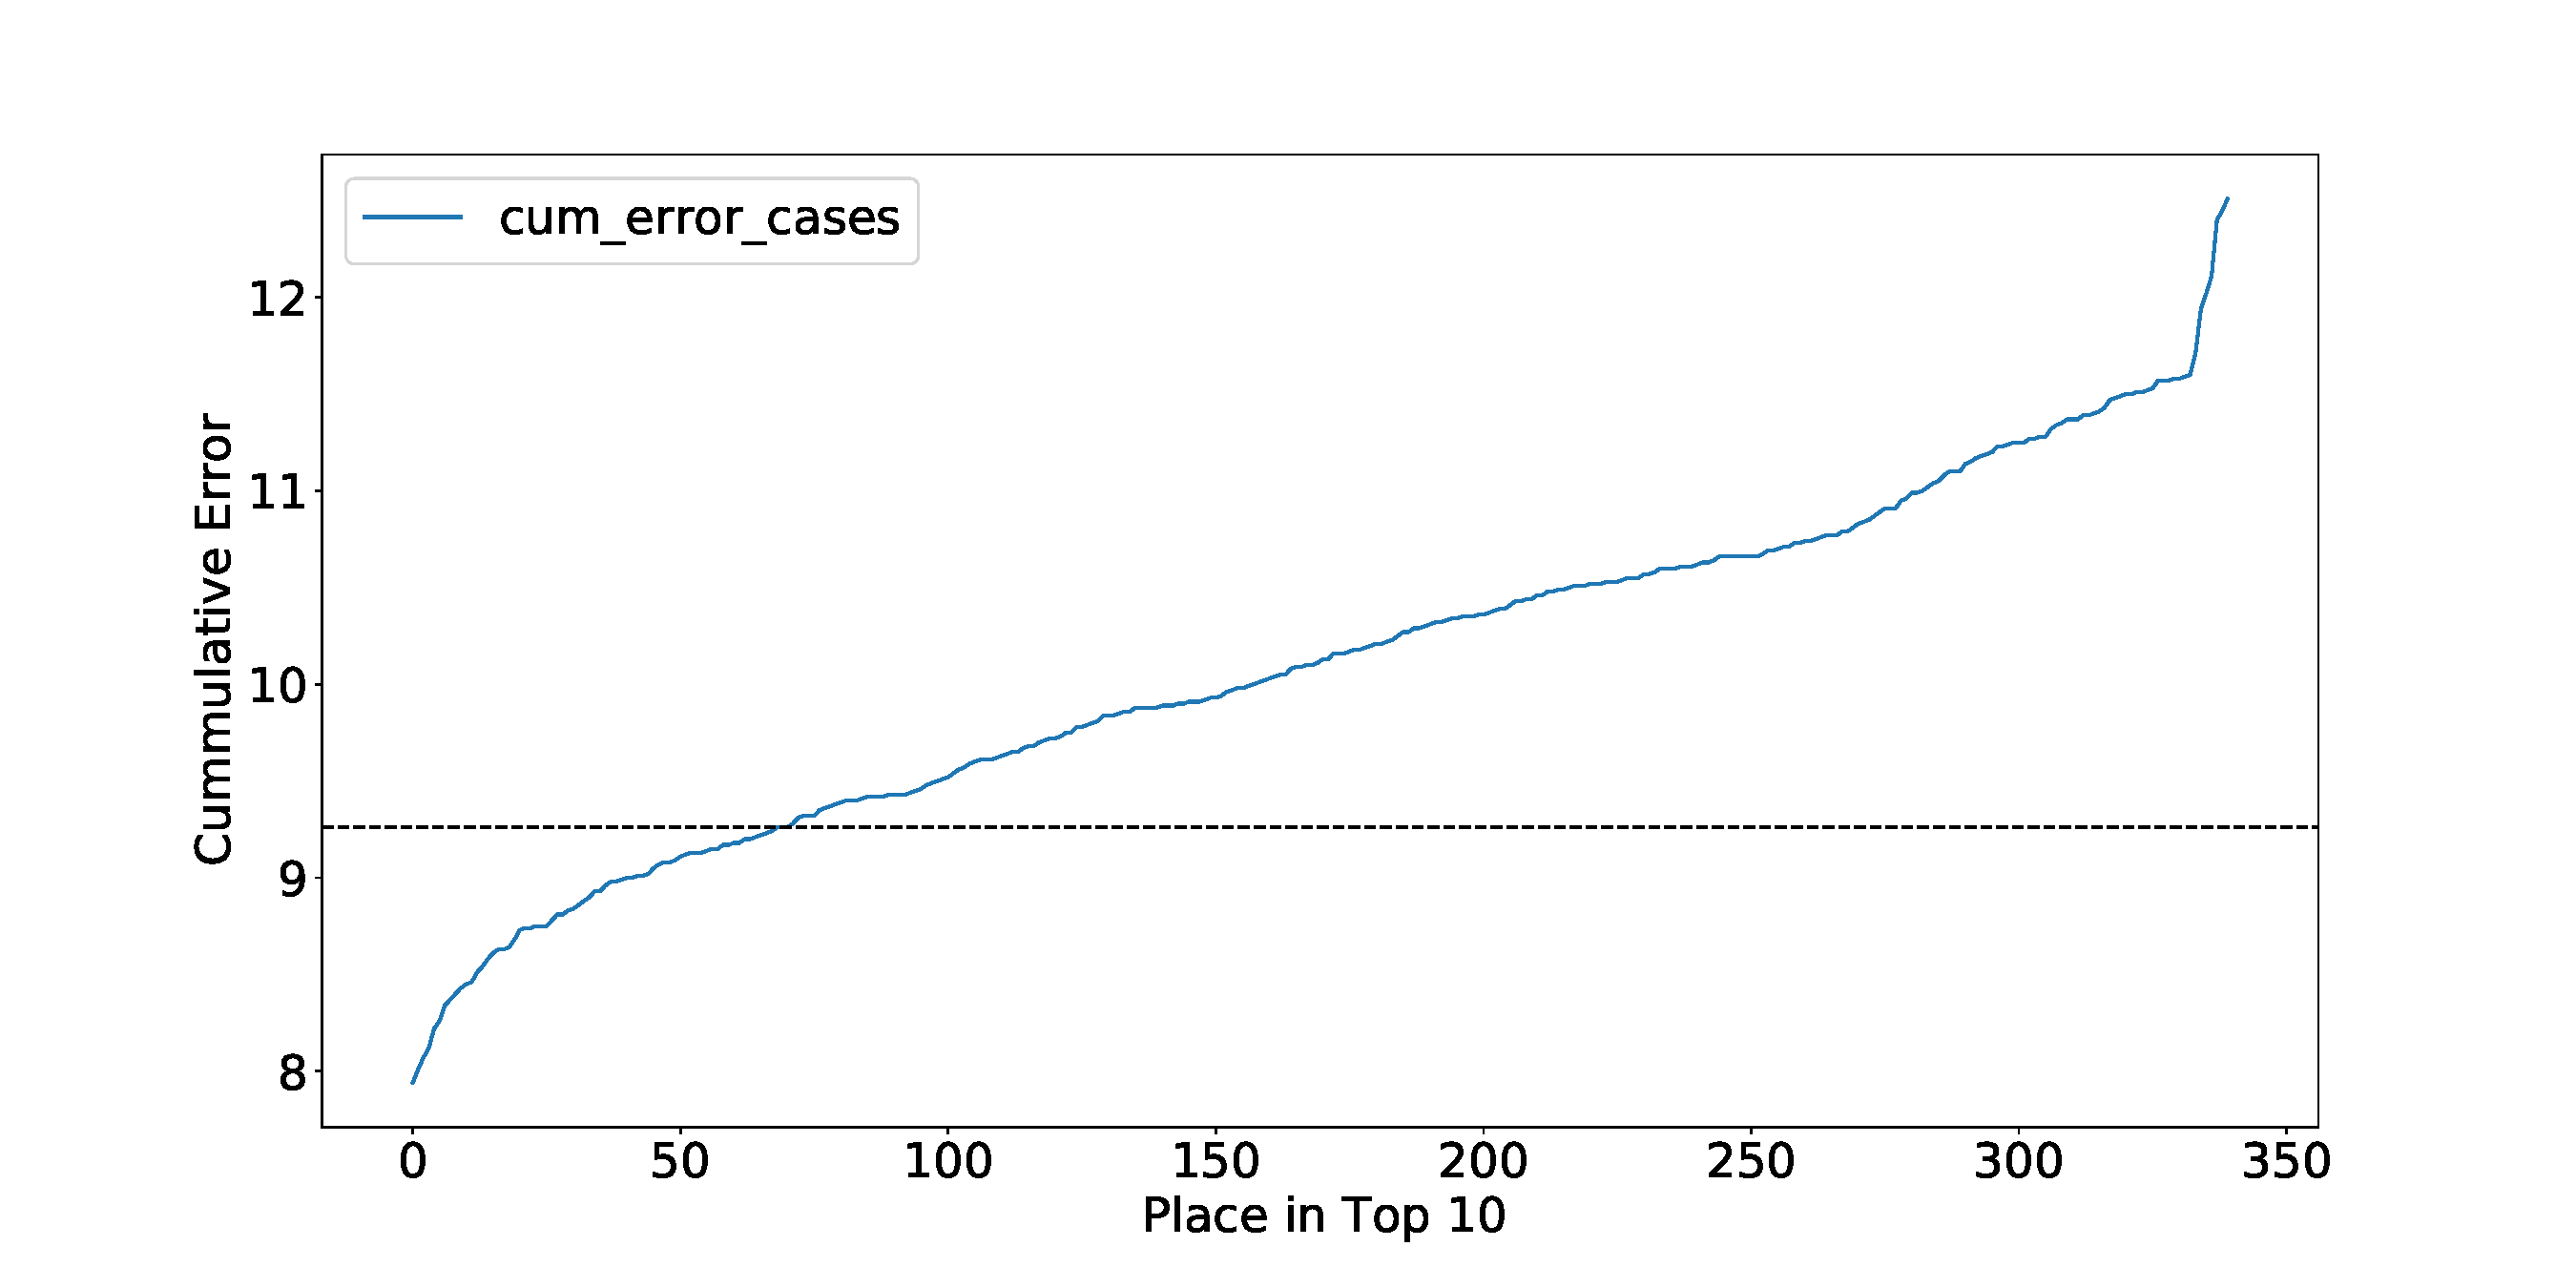
\includegraphics[width=1.0\textwidth]{images/predict/PlaceTop10_Cases.pdf}
        \caption{Cumulative error for cases}
        \label{fig:place-top10-cases}
    \end{subfigure}

    \caption{Top 10 predictions from all different risk factors sorted by cumulative error for deaths (\ref{fig:place-top10-death}) and cases (\ref{fig:place-top10-cases}). The horizontal line in each figure represents the model cumulative error with no risk factor as input for deaths and cases respectively.}
    \label{fig:place-top10-both}
    
    
\end{figure}



\begin{comment}

\subsection{Impact and Design of a Multi-Covariate-LSTM}
\label{sec:lstm-many}

In our next comprehensive analysis, we try to answer Question
\ref{q:4} if all risk factors impact the analysis. Thus we feed the
covariates into the recurrent network as additional features. In
addition to cases and deaths, this leads to 35 variables, including 33
unique covariates. We looked at two related ways of doing this: (a)
have covariates fixed in time (static), and (b) multiply the
covariates by the times series (we used the average of cases and
deaths)

We expected the second choice to be the most natural as it gives all
35 input streams similar time dependence. However, in our initial
tests, we found these choices gave very similar results, and so we
focused on the simpler choice (a) in this paper. In the experiments
discussed here, we either used 0, 1, or 33 covariates. Choosing 33
gives the best description (reducing loss by about 1\%) while using
each covariate as a solitary extra feature allows us a rather
sensitive study of the importance of each individual covariate as we
noted in Section \ref{sec:lstm-covariate}.

The final choice was the quantities to predict and train on. We choose
this to be both the cases and deaths values at the time value
following the sequence combined with the same quantities for the
following 14 days. This gives us 30 different output features for each
sequence. We renormalized, so the two basic features (following day)
contributed 50\% of the loss function. We supported this in TensorFlow
with a custom mean square error (MSE) loss function that dropped
training values that were not available for time sequences near the
end of the examined period. While one can not train on future values,
we can predict them, as seen in our sample outputs. We extensively
studied both 2 and 30 output features, and they give similar
descriptions of the observed data with the 30 feature choice enabling
14-day predictions.

We performed an extensive hyper-parameter search and we show the
values in Table \ref{tab:model} that give robust results without
overfitting. Furthermore, we looked at four different activation
functions for this analysis in the LSTM and fully connected
layers. Scaled Exponential Linear Unit (SELU), REctified Linear Unit
(RELU) and TANH activations gave very similar results while SIGMOID
activation was much worse. However we still use a SIGMOID function in
the last stage just as we did in Section \ref{sec:lstm-covariate}. We
also looked at the number of hidden units (separately for LSTM and
fully connected layers), the number of LSTM layers and the dropout
values.  Only the latter produced a significant change and, for
example, removing dropouts decreased the loss by about 16\% but we
retained them to provide a robust environment. We chose randomly 20\%
of the data for validation and testing and this had similar loss
values to the training data (the other 80\%) with our chosen dropout.

The final technical issue concerns the data normalization where each
feature is transformed by a feature dependent -- but city independent
-- way to lie between 0 and 1. Further all extensive (proportional to
size) covariates were first divided by the city population except for
the population itself where we took the logarithm; intensive
covariates were just rescaled to lie between 0 and 1. The basic
COVID-19 daily data is extensive but compared two approaches with and
without renormalization, but in this case, we took the square root of
the data value.  This is natural if there are counting (square root(N)
for N observations) errors as the deep learning loss function is
$(predicted-observed)^{2}$ without the error traditional in
$\chi^{2}$, namely $((predicted-observed)/error)^{2}$. This approach
with standard deep learning MSE appears sound instead of dividing by
the population. That will emphasize the error contribution of smaller
cities but is still interesting to look at due to the presence of many
systematic errors.


\section{Direct Deductions from Deep Learning Data Representation}

The deep learning model contains a lot of information much of which we
have already analyzed and discussed in Section
\ref{sec:lstm-covariate} and Figures \ref{fig:magic-1} and
\ref{fig:error-case-popdensity}. In addition, we have looked at the
sensitivity of the results as measured by the predicted daily rates
and the value of the loss function. In Table \ref{tab:corr-matrix}, we
present one way of looking at it. We calculate the correlation
coefficients of many of the covariates from an accurate LSTM model fit
to the data. We divide the time series into three regions

\begin{itemize}
\item \textbf{Past} or all days up to 14 days before the final
  observed date (May 25, 2020)
\item \textbf{Now} or the 14 days from May 12 to May 25, 2020
\item \textbf{Future} or the 14 days after May 25, 2020 predicted by
  the model
\end{itemize}
 
These results are different between population normalized or direct
non-normalized data. We have kept the square-root used in the model
but divided the model values by the square root of the population when
computing the correlation. Significant positive correlations are seen
for CASTHMA, HIGHCHOL, DIABETES, OBESITY, CSMOKING, CHD, and CHECKUP ,
while negative correlations for PVI and NORM\_POP. We also looked at
the impact of these covariates on the evolution function. As this
operates on data at previous time values, this is sensitive to
variations across cities and times. The evolution operator is
intuitively the time derivative of the absolute values of daily rates
seen in the correlation in Table 3. Nhosp and Estbeds have the most
significance in impacting (as a reduction) the values of both the
infection and fatality rates from the evolution operator. The fatality
rates are also significantly impacted by INSURANCE and NORM\_POP
(reduction) and SENIOR and OBESITY (increase) from the evolution
operator. NORM\_POP impacts infection values as an increase.  We can
also identify which covariates have the most significant impact on the
loss function. Here NHOSP, CHD, KIDNEY, BINGE, and PHLTH give 5\% or
more reduction in loss function while NORM\_POP, SVI\_OVERALL,
CASTHMA, DIABETES, and BPHIGH have small (1\%) effects.


\begin{table}[!h]
\caption{Correlation Matrix}
\bigskip
\label{tab:corr-matrix}
\begin{center}
\begin{tabular}{lrrrrrr}
\toprule
Risk Factor		&
\makecell{Past\\Case} &
\makecell{Now\\Case} &
\makecell{Future\\Case} &
\makecell{Past\\Death} &
\makecell{Now\\Death} &
\makecell{Future\\Death} \\
\midrule
PVI                     & -0.425      & -0.292      & -0.124      & -0.434      & -0.373      & -0.239    \\
INSURANCE               & 0.018       & 0.017       & 0.012       & 0.018       & -0.002      & 0.001     \\
NBEDS                   & 0.136       & 0.131       & 0.217       & 0.089       & 0.080        & 0.109     \\
NBEDS/1000              & 0.138       & 0.121       & 0.209       & 0.092       & 0.069       & 0.088     \\
NHOSP                   & 0.074       & 0.119       & 0.165       & -0.009      & 0.028       & 0.021     \\
ESTBEDS                 & 0.136       & 0.131       & 0.217       & 0.089       & 0.080        & 0.109     \\
SENIOR                  & 0.104       & 0.028       & 0.033       & 0.152       & 0.164       & 0.156     \\
BLACK                   & 0.209       & 0.099       & 0.208       & 0.216       & 0.085       & 0.116     \\
HISPANIC                & -0.072      & -0.032      & -0.064      & -0.091      & -0.068      & -0.046    \\
POP\_DENSITY\_2010      & -0.302      & -0.210      & -0.175      & -0.272      & -0.231      & -0.216    \\
POVERTY                 & 0.128       & 0.059       & 0.200       & 0.148       & 0.031       & 0.080     \\
SVI\_MINORITY           & 0.029       & 0.069       & 0.081       & 0.010        & 0.006       & 0.087     \\
SVI\_OVERALL            & 0.140       & 0.158       & 0.238       & 0.125       & 0.113       & 0.179     \\
CASTHMA                 & 0.238       & 0.271       & 0.307       & 0.205       & 0.288       & 0.309     \\
HIGHCHOL                & 0.202       & 0.185       & 0.131       & 0.192       & 0.243       & 0.224     \\
DIABETES                & 0.200       & 0.200     & 0.178         & 0.206       & 0.232       & 0.230     \\
OBESITY                 & 0.199       & 0.205       & 0.194       & 0.191       & 0.229       & 0.212     \\
CANCER                  & -0.145      & -0.102      & -0.129      & -0.138      & -0.058      & -0.059    \\
STROKE                  & 0.123       & 0.125       & 0.117       & 0.167       & 0.143       & 0.135     \\
MHLTH                   & 0.110       & 0.161       & 0.186       & 0.076       & 0.175       & 0.222     \\
CSMOKING                & 0.189       & 0.258       & 0.249       & 0.160        & 0.289       & 0.323     \\
CHOLSCREEN              & 0.164       & 0.001       & -0.026      & 0.187       & 0.070       & 0.038     \\
INSURANCE               & 0.018       & 0.017       & 0.012       & 0.018       & -0.002      & 0.001     \\
CHD                     & 0.225       & 0.284       & 0.233       & 0.178       & 0.327       & 0.337     \\
CHECKUP                 & 0.206       & 0.221       & 0.280       & 0.201       & 0.272       & 0.343     \\
KIDNEY                  & 0.045       & 0.028       & 0.032       & 0.022       & 0.071       & 0.053     \\
BINGE                   & 0.031       & 0.044       & 0.009       & 0.083       & 0.030       & 0.022     \\
LPA                     & 0.191       & 0.187       & 0.197       & 0.147       & 0.220       & 0.214     \\
ARTHRITIS               & 0.046       & 0.013       & -0.021      & 0.061       & 0.089       & 0.079     \\
BPMED                   & 0.060       & 0.080        & 0.124       & 0.056       & 0.073      & 0.090      \\
PHLTH                   & 0.064       & 0.132       & 0.104       & 0.022       & 0.129       & 0.114     \\
BPHIGH                  & 0.056       & 0.051       & 0.048       & 0.058       & 0.084       & 0.068     \\
COPD                    & 0.163       & 0.163       & 0.153       & 0.175       & 0.220       & 0.240     \\
NORM\_POP               & -0.305      & -0.258      & -0.218      & -0.193      & -0.218      & -0.099  \\
\bottomrule
\end{tabular}
\end{center}
\end{table}

\end{comment}


\section{Conclusion}

While this study focuses on if and which risk factors can improve the
predictions, we do not focus on why. Such analysis could provide
insights into causal relationships. For example, information such as
health insurance and the number of hospitals and beds are often
related to the quality of services that affect early detection and
treatment. Furthermore, population parameters such as population density can
determine the rate of spread and the number of cases. Similarly,
distributions of comorbidities in a given population such as physical
health, cholesterol screening, diabetes, etc., are found to be
insightful in predicting outcomes \citep{Maleki}. Identifying such risk
factors and correlating them to the prediction accuracy provides
valuable candidates for future studies.

A variety of mathematical and computational models have been used for
predicting COVID-19 outcomes \citep{Jewell}. It includes compartmental
models such as the SIR (Susceptible-Infected-Recovered) and SEIR
(Susceptible-Exposed-Infected-Recovered) which are relatively easy to
compute, and thus, commonly used in epidemiology. However, their
simplistic assumptions, such as homogeneous mixing within populations,
might make them less realistic for pandemics such as COVID-19. For
instance, such models often assume a closed population that does not
change. However, COVID-19 dynamics have prominently included massive
migration, deaths due to comorbidities temporarily conferred immunity,
and notably, major disparities in terms of socio-economic determinants
of health.

In terms of implementation, SIR and SEIR models are fitted with point
estimates, which may not adequately reflect the disease dynamics. For
instance, it is difficult to account for behavioral changes (e.g.,
human mobility) or systemic inadequacies (e.g., availability of
hospital beds) that may appear in specific subpopulations. Finally,
the compartmental model estimates do not allow for quantification of
uncertainty, which makes it harder to use them in policy-making. A
comparison of modeling approaches concluded that while SEIR model
performed better for a couple of states in the U.S., alternatives have
performed better for the other states \citep{Bertozzi}. AICov has
addressed most of the above modeling issues in its design, as per the
requirements of its forecasting objectives.

We present AICov as an integrative deep learning framework for
COVID-19 forecasting with the help of population covariates. Thus, its
objectives are different from those of traditional compartmental
models. One of the important features of the architecture for AICov is
that it is by design targeting Cloud and High Performance Computing
(HPC) resources to conduct parameter sweeps to leverage sophisticated
deep learning toolkits. The architecture allows the integration of
various data sources that can update the data from its sources on
demand and update its model predictions based on newly introduced
data. Parameters can easily be adjusted via Jupyter notebooks that, in
turn, call the computational backends on HPC and cloud resources.

In addition to this architecture, we used data collected from multiple
public sources and agencies, and integrated the same across spatially
contiguous units such as cities or metropolitan areas. In our
analysis, we have focused on 110 selected cities of the U.S., but the
framework is general and can be used to analyze similar data on
pandemics from anywhere in the world.

The comprehensive analysis showcases the feasibility of our
approach. Based on the outcomes reported it can lead to an improved
prediction once we integrate risk factors in addition to the
time-dependent data such as cases and death resulting from
COVID-19. While the improvements observed were modest, they do present
a concrete way of improving the forecast models. Inclusion of further
putative factors from the ongoing worldwide studies on Covid-19 will
only strengthen the future applications of our integrative framework.

We have shown that deep learning can return very good results while
using smooth data, which we used in our empirical fits. For real data
as presented to us for the daily changes, it still produced good
results and even was able to predict changes based on weekly
fluctuations. This is typically not achieved by other non-data based
model approaches. Also, we have used in our data only cases and
deaths, but we intend to expand this by using data about recovery and,
in the future, immunization.

We have experimented with different hyperparameters and included in
this study a selection of hyperparameters that have worked well for
this data set.


As we have set up the first version of our AICov software, we have
used cloud and high-performance computers. All of our sophisticated
analyses were run in a day on at most 16 computers. All deep learning
algorithms that were run on GPUs were run on NVIDIA Tesla
K80s. However, our framework is on purpose generalized so that other
compute resources can be integrated and leveraged. This includes
local, HPC, and cloud computing resources, as well as different
GPUs. Naturally, we also need to take into consideration not only the
compute time but also the time it takes for the researcher to derive
the models. As our approach is self-learning based on automated data
updates, the time to prepare an updated model can be automatized and
minimal input is needed. Thus the overall effort is very competitive.



\begin{comment}
Furthermore, we are currently conducting experiments with multiple
risk factors at the same time to identify the most significant
combinations of them.  As we have shown that the bivariate analysis
has a locality dependency, we will explore categorizing locations with
similar demographics and conduct further experiments on demographical
similar regions.
\end{comment}

%%%%%%%%%%%%%%%%%%%%%%%%%%%%%%%%%%

%
% SUPLEMENTAL
%

\section*{Supplementary Materials}

The code and paper document represented to implement AICov are contained in several repositories:

\begin{enumerate}
    \item The entire cloudmesh code on which the cloud based implementation of the AICov framework is based and contains over 70 contributors is available publicly at \url{https://github.com/cloudmesh}. Cloudmesh contains a number of modules that dependent on the users access to cloud resources can be customized. A detailed manual about the configuration is available at \url{https://cloudmesh.github.io/cloudmesh-manual/}.
    
    \item The entire COVID-19 analysis leverages cloudmesh and uses Jupyter notebooks to coordinate its workflow as discussed in the architecture Figure \ref{fig:arch}. The code and data for the results presented in this paper are located in the repository at \url{https://github.com/cloudmesh/cloudmesh-covid}.
    
    The data was analysed on a variety of supercomputing resources including an allocation of 20 compute nodes that were utilized to execute the  repeated model creation to assure reproducible results.
    
    However, as a publication is pending, at this time, the use of the data is copyrighted and can not be used for other publications without contacting the authors. The data gathering and analysis is a significant intellectual contribution and we like to avoid that the data is taken before we have not secured a publication. 
    
    \item The entire paper is located in \LaTeX source in the github repository \url{https://github.com/cyberaide/paper-covid}. This repository will be open sourced after acceptance of publication to not violate any publisher restrictions. If desired the authors can grant access to this repository prior to publication. Please contact the corresponding author.
    
\end{enumerate}

%
% ACKNOWLEDGMENT
%

\section*{Acknowledgements}

This work is partially supported by the National Science Foundation
(NSF) through awards Cyberinfrastructure Framework for 21st Century
Data Infrastructure Building Blocks (1443054), Network for
Computational Nanotechnology Engineered nanoBIO Node (1720625),
Cybertraining (1829704), CyberInfrastructure for Network Engineering
and Science (1835598) and Global Pervasive Computational Epidemiology
(1918626).  We thank J. Kadupitiya for several useful discussions on
deep learning frameworks.

\clearpage

\section*{Acronyms}

This section contains the list of acronyms in Table \ref{tab:acronyms}
as used in the paper for easy reference. The definitions of the risk
factors are however given within the paper in
Table~\ref{tab:risk-factors} on page \pageref{tab:risk-factors} and
not repeated here.

\begin{table}[!h]
  \caption{Non-risk factor acronyms used in this paper.}
  \label{tab:acronyms}
  \begin{tabular}{ll}
    \toprule
    Abbreviation & Description \\
    \midrule
    API & Application Programming Interfaces \\
    BRFSS & Behavioral Risk Factor Surveillance System \\
    CDC & U.S.~Centers for Disease Control and Prevention \\
    CI & Continious INtegration \\
    COVID-19 & COrona VIrus Disease 2019  \\
    CSSE & Center for Systems Science and Engineering \\
    cum & cumulative \\
    FIPS & Federal Information Processing Standards \\
    GPUs & Graphics Processing Units  \\
    HPC & High Performance Computing \\
    LSTM & Long Short-Term Memory \\
    MSE & Mean Squared Error \\
    NBDIF & NIST Big Data Working Group \\
    NCHS & CDC National Center for Health Statistics \\
    NIST & National Institute of Standards and Technology \\
    NONE & No risk factors used \\
    NORM\_POP & Normalized Population \\
    NSF & National Science Foundation \\
    RELU & REctified Linear Unit \\
    REST & REpresentational State Transfer  \\
    RMSE & Root Mean Squared Error \\
    RNN & Recurrent Neural Network \\
    SEIR & Susceptible, Expose, Infectious, Recovered) \\
    SELU & Scaled Exponential Linear Unit \\
    SIR &  Susceptible, Infectious, Recovered \\
    U.S. & United States of America \\
    WHO & World Health Organization \\
    \midrule
  \end{tabular}
\end{table}

\clearpage


\bibliographystyle{jdsurl}
\bibliography{bib/data-covid19,bib/lstm,bib/cloudmesh}


\end{document}
